\documentclass[english,twoside,openright]{HYgradu}
\usepackage{Preamble}
\graphicspath{{./figures/}}

% Add subfigure
\newcommand{\minifig}[1]{  
   \begin{minipage}[c]{0.3\linewidth}
      \centering
      \includegraphics[width=1.1\linewidth]{#1} 
      \vspace{0mm}
  \end{minipage}
}

% Add subfigure with text overlay
\newcommand{\minifigii}[4]{
   \begin{minipage}[c]{0.38\linewidth}
  	\begin{picture}(100,160)
		\put(0,0){\includegraphics[width=1.15\linewidth]{#1} }
		\put(#3,#4){\small{\textbf{#2}}}
	\end{picture} 
    \end{minipage}
}
%-------------------------------------------------------------------------------
% HEADER & FOOTER
%-------------------------------------------------------------------------------
%\fancyhf{}
%\fancyhead[L]{Otto Lindblom}
%\fancyhead[R]{014447947}
%\fancyfoot[R]{Sida \thepage\ av \pageref{LastPage}}

%-------------------------------------------------------------------------------
% TITLE PAGE & ABSTRACT PAGE
%-------------------------------------------------------------------------------
\title{A Computational Study of Isotope Exchange as a Tritium Removal Tool in Tungsten}
\author{Otto Lindblom}
\date{November 20, 2020}
\level{Master's thesis}
\subject{Computational Physics}
\faculty{Faculty of Science}
\programme{Computational Physics}
\department{Department of Physics}
\keywords{hydrogen, tritium, isotope exchange, molecular dynamics, tungsten}
\address{P.O. 64 (Gustaf H\"{a}llstr\"{o}ms gata 2a)\\00014 University of Helsinki}
\prof{Dr. Tommy Ahlgren}
\censors{Prof. Kai Nordlund}{Dr. Tommy Ahlgren}{}
\depositeplace{Kumpula Science Library}
\additionalinformation{}
\classification{}

% if you want to quote someone special. You can comment this line and there will be nothing on the document.
%\quoting{Bachelor's degrees make pretty good placemats if you get them laminated.}{Jeph Jacques} 

\begin{document}

% Generate title page.
\maketitle

% English abstract

\begin{abstract}
Due to its exceptional thermal properties and irradiation resistance, tungsten is the material of choice for critical plasma-facing components in many leading thermonuclear fusion projects.
Owing to the natural retention of hydrogen isotopes in materials such as tungsten, the safety of a fusion device depends heavily on the inventory of radioactive tritium in its plasma-facing components. 
The proposed methods of tritium removal typically include thermal treatment of massive metal structures for prolonged timescales.
A novel way to either shorten the treatment times or lower the required temperatures is based performing the removal under an H$_2$ atmosphere, effectively exchanging the trapped tritium for non-radioactive protium. 

In this thesis, we employ molecular dynamics simulations to study the mechanism of hydrogen isotope exchange in vacancy, dislocation and grain boundary type defects in tungsten.
By comparing the results to simulations of purely diffusion-based tritium removal methods, we establish that hydrogen isotope exchange indeed facilitates faster removal of tritium for all studied defect types at temperatures of 500 K and above.
The fastest removal, when normalising based on the initial occupation of the defect, is shown to occur in vacancies and the slowest in grain boundaries.   
Through an atom level study of the mechanism, we are able to verify that tritium removal using isotope exchange depends on keeping the defect saturated with hydrogen.

This study also works to show that molecular dynamics indeed is a valid tool for studying tritium removal and isotope exchange in general. 
Using small system sizes and spatially-parallelised simulation tools, we have managed to model isotope exchange for timescales extending from hundreds of nanoseconds up to several microseconds.
\end{abstract}


% Swedish abstract
\date{20.11.2020}
\level{Magistersavhandling}
\subject{Beräkningsfysik}
\faculty{Matematisk-naturvetenskapliga fakulteten}
\programme{Beräkningsfysik}
\department{Avdelningen för fysik}
\keywords{väte, tritium, isotopbyte, molekyldynamik, wolfram}
\depositeplace{Vetenskapsbiblioteket i Gumtäkt }
\additionalinformation{}
\classification{}
\begin{abstract}
Tack vare sina exceptionella termiska egenskaper samt strålningsuthållighet, har  wolfram valts som material för kritiska, plasmariktade komponenter i flera ledande termonukleära fusionsprojekt.
Eftersom väteisotoper naturligt uppfångas av material som wolfram, beror säkerheten på fusionsanordningar i hög grad på mängden kvarhållet tritium i dess komponenter.
De föreslagna metoderna för avlägsning av tritium inkluderar vanligen termisk behandling av massiva metallstrukturer under långa tidsskalor. 
En nyare metod, som möjliggör antingen en förkortning av behandlingstiderna eller en sänkning temperaturen, går ut på att behandlingen görs under en H$_2$-atmosfär.
Detta baserar sig i praktiken på att det infångade tritiumet byts ut mot icke-radioaktivt protium.

I denna avhandling, använder vi oss av molekyldynamiska simulationer för att studera mekanismen bakom väteisotopbytet i vakanser, dislokationer samt korngränser i wolfram.
Genom att jämföra resultaten med simulationer av rent diffusionsbaserade behandlingsmetoder, framhåller vi att isotopbytet försnabbar avlägsningen av tritium i alla granskade defekttyper vid 500 K och högre temperaturer.
Den snabbaste avlägsningen visas ske i vakanser och långsammaste i korngränser, då vi normaliserar avlägsningsraterna baserat på den ursprungliga mängden tritium i defekten.
Med hjälp av en analys av mekanismen på atomnivå, kan vi bekräfta att tritiumavlägsning via isotopbyte baserar sig på att hålla defekten saturerad med väte.

Denna studie visar även att molekyldynamiska metoder lämpar väl sig för simulering av tritiumavlägsning samt isotopbyte i allmänhet.
Genom att använda småskaliga system, har vi lyckats simulera isotopbyte under tidsskalor som sträcker sig från hundratals nanosekunder upp till flera mikrosekunder.
\end{abstract}

% Finnish abstract
\date{20.11.2020}
\level{Maisterin tutkinto}
\subject{Laskennallinen fysiika}
\faculty{Matemaattis-luonnontieteellinen tiedekunta}
\programme{Laskennallinen fysiika}
\department{Fysiikan osasto}
\keywords{vety, tritium, isotooppivaihto, molekyylidynamiikka, volframi}
\depositeplace{Kumpulan tiedekirjasto }
\additionalinformation{}
\classification{}
\begin{abstract}
Poikkeuksellisista lämpöominaisuuksistaan sekä säteilykestävyydestään tunnettu volframi on valittu useiden uraauurtavien fuusioprojektien kriittisten, plasmanvastaisten komponentien materiaaliksi.
Johtuen vedyn isotooppien luontaisesta kerääntymisestä materiaaleihin kuten volframi, fuusiolaitteiden turvallisuus riippuu ratkaisevalla tavalla laitteen komponenttien sisältämän tritiumin määrästä.
Tritiumin poistamiseksi kaavailtuihin menetelmiin sisältyy tyypillisesti valtavien metallikomponenttien pitkäkestoinen lämpökäsittely.
Uudenlainen menetelmä, joka perustuu komponenttien käsittellyyn H$_2$-ilmakehässä, mahdollistaa kuitenkin käsittelyn joko lyhyemmässä ajassa tai matalammissa lämpötiloissa.

Tässä tutkielmassa hyödynnämme molekyylidynaamisia simulaatioita vetyisotooppivaihtomekanismin tutkimiseksi volframin vakansseissa, dislokaatioissa sekä raerajoissa.
Vertaamalla tuloksiamme puhtaasti diffuusioon perustuvia käsittelymenetelmiä kuvaaviin simulaatioihin, osoitamme isotooppivaihdon nopeuttavan tritiumin poistumista kaikissa tarkastelluissa kidevirhetyypeissä 500 K:ssä ja sitä korkeammissa lämpötiloissa.
Osoitamme tritiumin poistuvan nopeimmiten vakansseista ja hitaimmiten raerajoista kun poistumisnopeus suhteutetaan kidevirheessä alunperin olevan tritiumin määrään. 
Tarkastelemalla ilmiötä atomitasolla, voimme vahvistaa isotooppivaihdon kautta tapahtuvan tritiumin poiston perustuvan  kidevirheen pysymiseen vedyllä saturoituneena. 

Tämä tutkielma pyrkii myös osoittamaan molekyylidynamiikan käyttömahdollisuudet tritiumin poiston sekä isotooppivaihdon simuloimisessa.
Käyttämällä pienikokoisia järjestelmiä, olemme onnistuneet simuloimaan isotooppivaihtoa sadoista nanosekunneista useaan mikrosekunttiin ulottuvilla aikaskaaloilla.
\end{abstract}

% Place ToC
\mytableofcontents

\mynomenclature
%\printnomenclature


%-------------------------------------------------------------------------------
% CONSTANTS, VARIABLES & ETC.
%-------------------------------------------------------------------------------
%\nomenclature{$p$}{Pressure \nomunit{atm}}
%\nomenclature{$V$}{Volume \nomunit{\AA$^3$}}
\nomenclature{$\delta_{\text{T}} $}{Normalised average tritium removal rate \nomunit{Atoms/ns}}
\nomenclature{$V$}{Potential energy \nomunit{eV}} 
\nomenclature{$\mathbf{r}_i$}{Position vector of $i$th atom \nomunit{\AA}}
\nomenclature{$\mathbf{F}_i$}{Force acting on $i$th atom \nomunit{ev/\AA}}
\nomenclature{$m_i$}{Mass of $i$th atom \nomunit{u}}
\nomenclature{H}{Protium atom}
\nomenclature{T}{Tritium atom}
\nomenclature{$k_{\text{B}}$}{Boltzmann constant \nomunit{1.38$\times10^{-23}$ J/K}}
\nomenclature{$a$}{Lattice constant \nomunit{\AA}}
%\nomenclature{$a$}{Tungsten lattice contstant \nomunit{3.165 \AA}}
\nomenclature{$m_{\rm W}$}{Tungsten mean atomic mass \nomunit{183.85 u}}
\nomenclature{$m_{\rm H}$}{Protium mean atomic mass \nomunit{1.00784 u}}
\nomenclature{$m_{\rm T}$}{Tritium mean atomic mass \nomunit{3.0161 u}}


%-------------------------------------------------------------------------------
% BODY
%-------------------------------------------------------------------------------

%--------------------------------------------------------------------

% ===================================================================================================
\chapter{Introduction}
% ===================================================================================================

Many fundamental challenges of our century can be linked to finding ways of meeting the globally increasing demand for sustainable energy. 
One viable solution to increasing the large scale production of clean energy is through the harnessing of thermonuclear fusion. 
In its most researched form, nuclear fusion consists of fusing two hydrogen isotopes, deuterium (D, $^2_1$H) and tritium (T, $^3_1$H), and thereby producing helium ($^4_2$He) and a neutron, in a process which releases large quantities of energy. 
Per unit of mass, the D-T reaction offers almost six orders of magnitude more energy than any chemical process, including the burning of fossil fuels, and three times more than fission of uranium-235 in a modern nuclear power plant.  

Most of the energy emitted from the D-T reaction is released as the kinetic energy of the neutron. 
The plasma-facing surfaces of a fusion reactor are therefore subject to a constant bombardment by neutrons moving at over 17 \% of the speed of light, having the potential to displace atoms from their lattice positions on impact and cause widespread crystallographic damage. 
Due to their electrical neutrality, neutrons interact only to a negligible degree with electrons, limiting their interactions with atoms to the highly improbable collisions with atomic nuclei. 
Neutrons can thus penetrate several meters into the reactor walls, extending the damage from the surface, deep into the bulk material. 

Chosen for its high resistance against erosion by energetic ions and neutrons, tungsten (W) is the primary armour material candidate for the divertor of the groundbreaking ITER tokamak being constructed in southern France \cite{hirai2013iter}. % [brief description of divertors and/or ITER?]
It has, however, been shown that hydrogen isotopes can easily diffuse deep into bulk W, while crystallographic defects, such as those produced by the neutron radiation, enhance the retention of hydrogen within the material. \cite{tanabe2014review} 
This trapping mechanism tends to lead to an accumulation of hydrogen, including the radioactive isotope tritium (T), from the fusion fuel into the plasma-facing reactor components, rendering them radioactive over time. 
The inventory of embedded tritium is, therefore, a critical safety concern, but also a matter of fuel economy, since tritium is extremely rare and among the most expensive substances found on Earth.

Proposed methods for T removal include thermal treating of the affected components until most hydrogen has been detrapped and removed through diffusion \cite{heinola2017long}, but also the use of high-power pulsed flashlamps \cite{gibson2005removal} or lasers \cite{skinner2008recent,de2017efficiency} to only locally heat the material. 
For example, in the case of ITER, the plan for T removal consists of vacuum annealing the first wall at 513 K and the divertor at 623 K \cite{pitts2011physics}, essentially heating the components long enough for the embedded hydrogen isotopes to diffuse out through the nearest surface.
In practice, however, this method involves heating massive metal objects -- the divertor alone being a multi-part component built up from 54 ten-tonne cassette assemblies -- to high temperatures for extended periods of time. 
Tests performed at the ITER-like JET reactor additionally suggest that annealing at the proposed temperatures for as long as 15 h, will likely result in the removal of only around 40 \% of the tritium inventory \cite{heinola2017long}. 

Conveniently, it has been shown \cite{alimov2011hydrogen, roth2013hydrogen, barton2014deuterium} that annealing under a H$_2$ atmosphere can achieve similar results of tritium removal, but at significantly lower temperatures. 
This method makes use of the spontaneous replacement of tritium with a cheaper and safer isotope, protium (H, $^1_1$H), in a process aptly referred to as 'isotope exchange'. 
Experiments conducted with the non-radioactive hydrogen isotope deuterium, have indicated a near-perfect D removal after 24 h of annealing at 520 K under a H$_2$ atmosphere, while a similar removal rate using traditional vacuum annealing would require temperatures of around 700 K. \cite{ahlgren2019hydrogen}

Experimental studies of hydrogen isotope exchange in tugsten have been conducted by e.g. Alimov \textit{et al.} \cite{alimov2011hydrogen}, Roth \textit{et al.}  \cite{roth2013hydrogen}, Barton \textit{et al.} \cite{barton2014deuterium} and Ahlgren \textit{et al.} \cite{ahlgren2019hydrogen}. 
The phenomenon has also been modelled on a macroscopic scale by Hodille \textit{et al.} \cite{hodille2016study} using Macroscopic Rate Equation models, based on experimental results as well as Density Functional Theory (DFT) data on the behaviour of hydrogen near tungsten monovacancies. 
The isotope exchange occurring around a single crystal defect is likely to occur on a timescale of nano- to microseconds, but such scales are far beyond the reach of current DFT methods, while tools such as Rate Equations lack the atomic level insight to the studied mechanism.

In this thesis, we therefore set out to study the isotope exchange mechanism on a microscopic scale, using molecular dynamics to simulate the interactions between hydrogen and various crystallographic defects in tungsten.
We begin with a glance at the background of thermonuclear fusion reactors and the materials used in such devices, before moving on to describe the central computational tools used in this work. 
We continue with an overview of the simulation setups for the various defect types and finally conclude with an analysis of the results.



%--------------------------------------------------------------------

% ===================================================================================================
\chapter{Theory}
% ===================================================================================================

% ---------------------------------------------------------------------------------------------------
\section{Magnetic Confinement Fusion}
% ---------------------------------------------------------------------------------------------------
At a subatomic level, nuclear fusion is governed by two separate fundamental interactions -- the electromagnetic force, which causes the positively charged protons of two nuclei to repel each other, and the residual strong force, which binds together protons and neutrons to form nuclei. 
Due to their small size and the low number of protons, nuclei of elements lighter than nickel and iron can overcome the electromagnetic repulsion barrier and fuse into a single nucleus, typically releasing orders of magnitude more energy than any process involving chemical bonds.

Since the nuclei have to be brought to within around $10^{-15}$ m from each other in order for the short-ranged strong interaction to outweigh the electromagnetic repulsion, the process of forcing together even the lightest nuclei requires substantial amounts of energy.  
At the cores of stars, the immense pressure combined with temperatures of the order of $10^6$ K brings hydrogen atoms close enough for some of them to cross the repulsion barrier through the quantum mechanical effect of tunneling \cite{clayton1983principles}.
Without the gravitational mass of a star compressing the fuel, however, we have to rely on various 'dirty tricks' to achieve conditions suitable for a self-sustaining fusion reaction. 
Magnetic Confinement Fusion (MCF), seen generally as the most promising of such tricks, exploits the fact that charged particles can be manipulated using magnetic fields. 
The fuel is heated to temperatures around $10^7$ K, at which point the electrons and nuclei of the fuel atoms will have separated, transitioning into plasma. 
The goal of current MCF projects is to be able to control the plasma using strong magnets, confining it to a limited volume and simultaneously preventing it from contacting the reactor walls.
The combination of extreme heat and confinement then provides an environment suitable for fusion to occur.

Research focusing on MCF has been conducted since the early 1950s, with multiple reactor designs, such as the stellarator, Z-pinch and levitated dipole, having been proposed throughout the years. 
The tokamak, currently seen as the most promising design for an MCF reactor, was initially developed and first constructed in the late 1950s by Soviet physicists \cite{tokamakorigins}. 
This reactor type is best described by its name, which is a Russian acronym for a "toroidal chamber with magnetic coils".
In Fig. \ref{fig:tokamak}, we have rendered a 3D schematic of a typical tokamak.

\begin{figure}[!ht]
\center
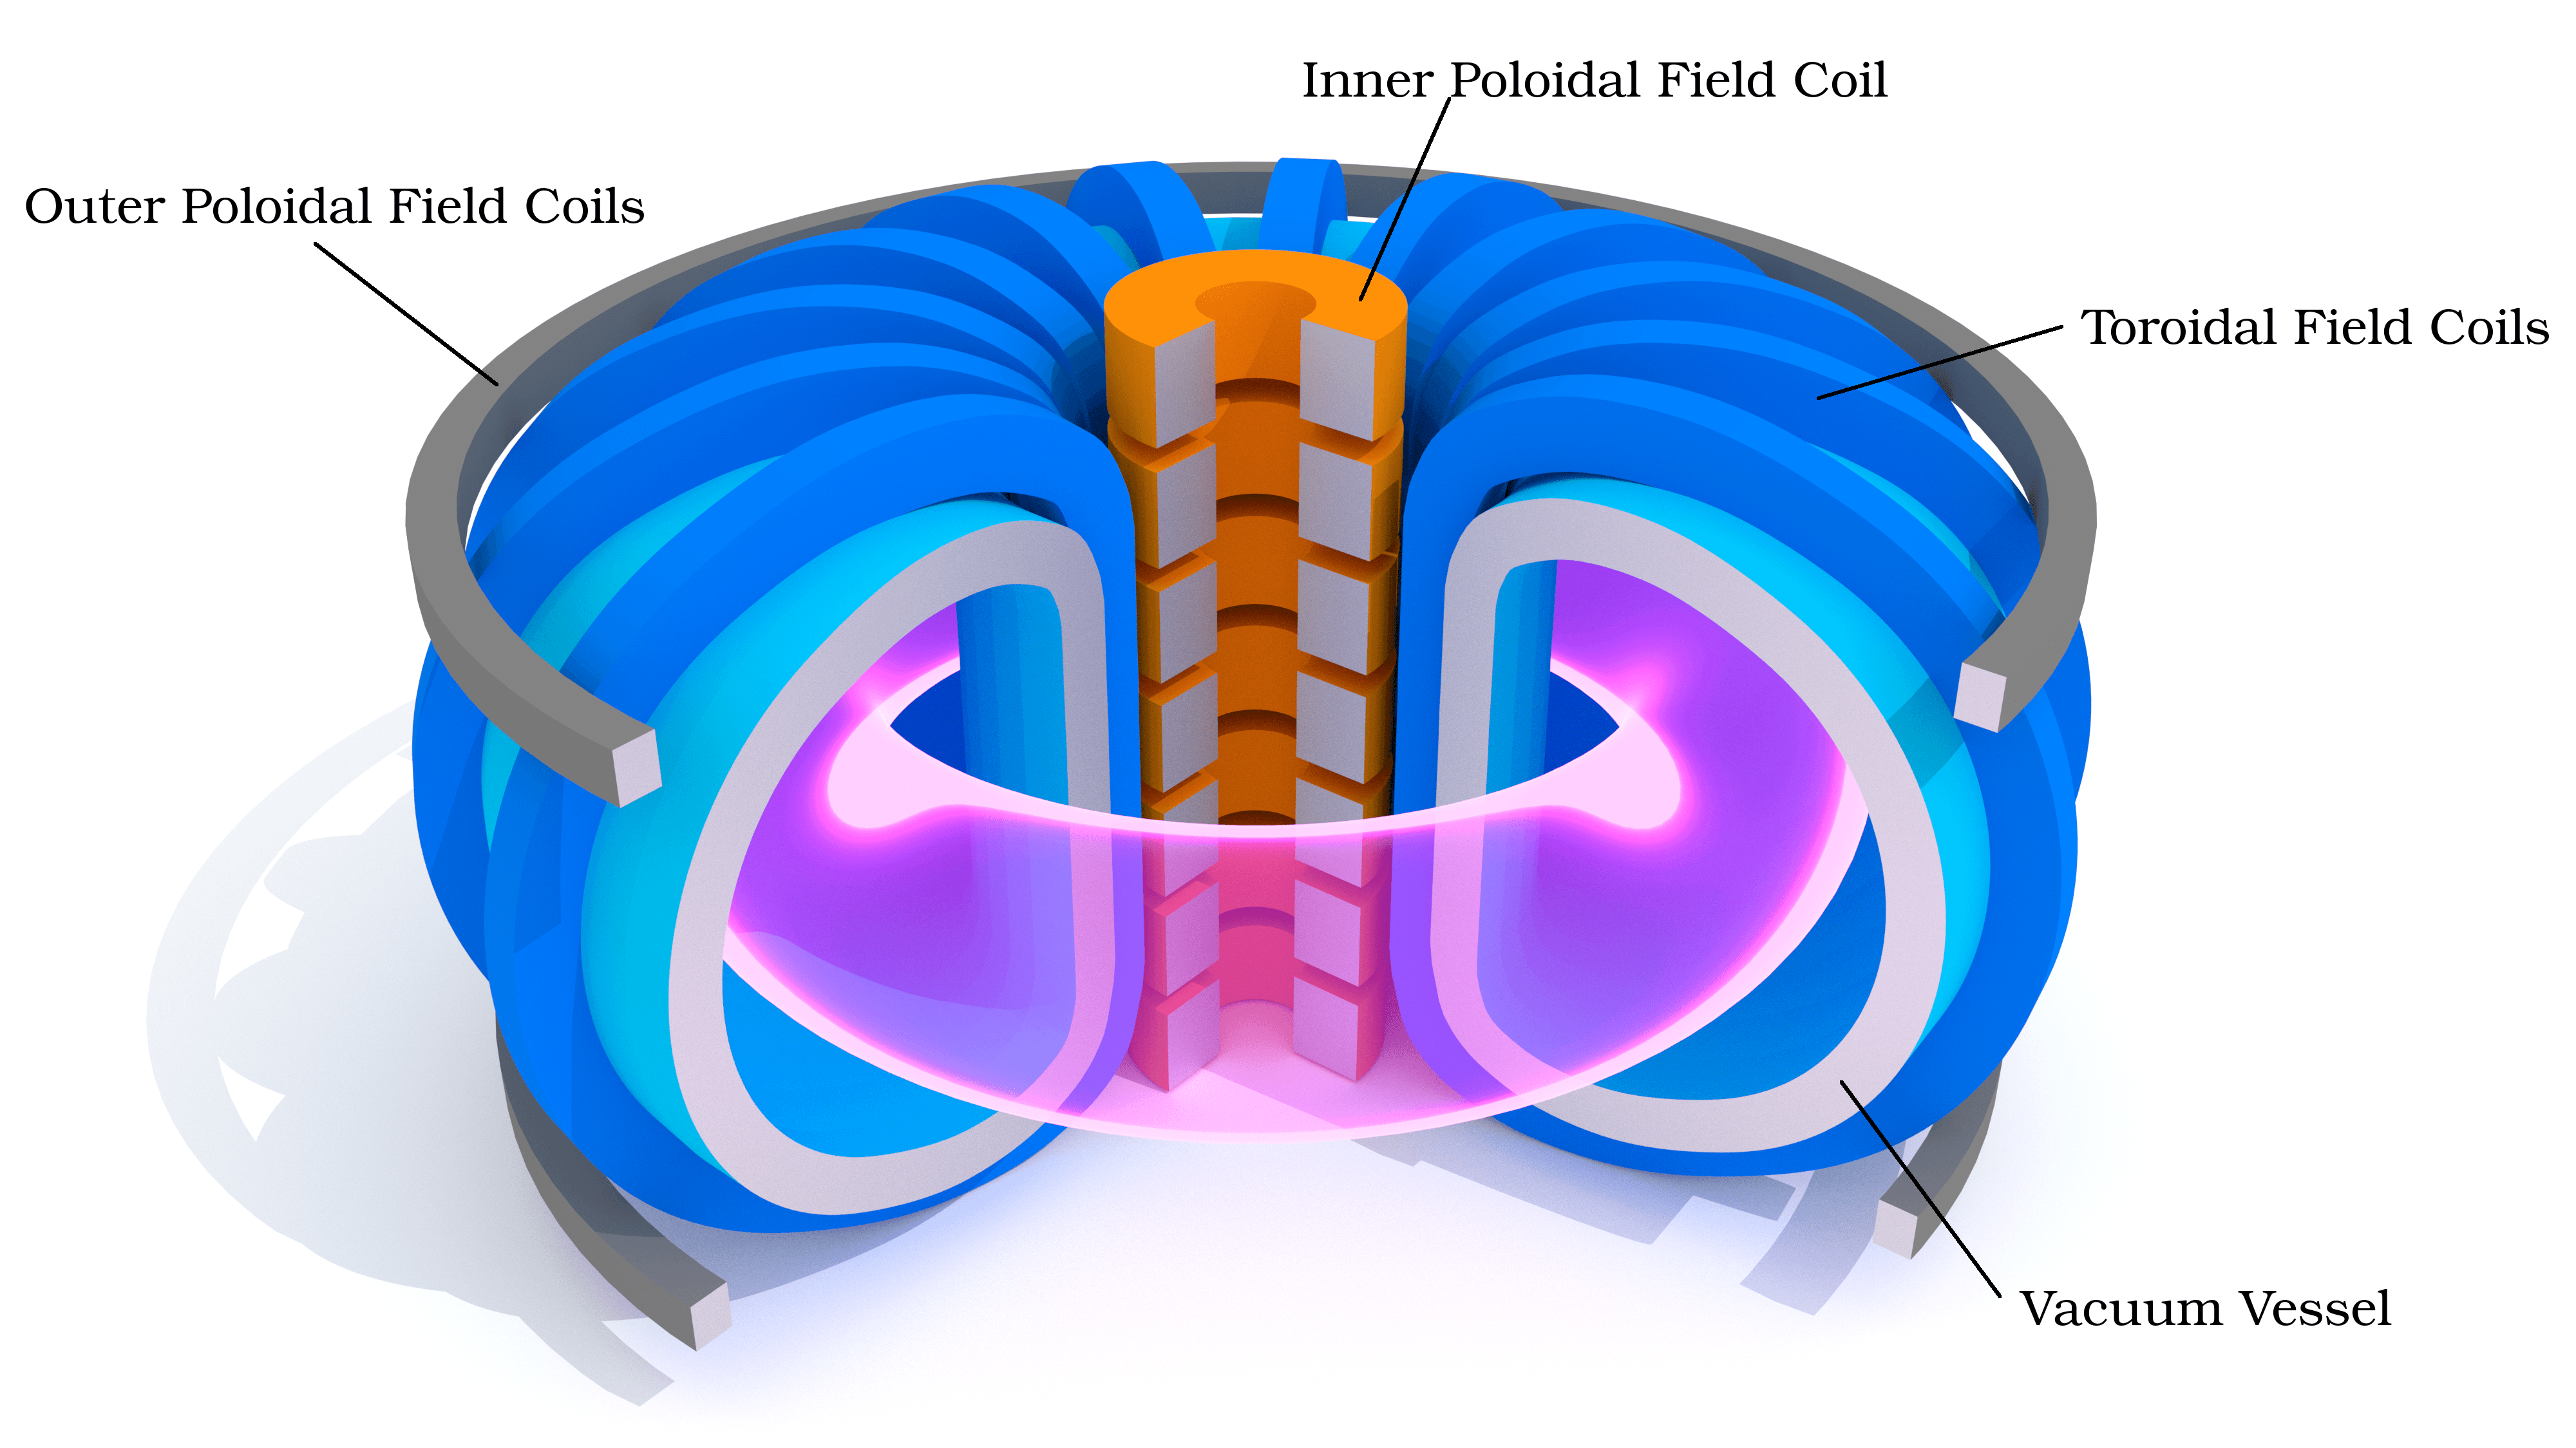
\includegraphics[width=0.8\linewidth]{Schematic-of-a-tokamak.png}
\caption{A schematic view of a tokamak-type fusion reactor.} 
\label{fig:tokamak}
\end{figure}

Regarding the fuel of an MCF reactor, any two light enough elements could in theory be fused. 
However, from a fuel-economical point of view, the deuterium-tritium reaction 
\begin{align}
^2_1\rm{H} ~+~ ^3_1\rm{H} ~\rightarrow~ ^4_2\rm{He} ~+~ ^1_0\rm{n} ~+~ 17.58 ~\rm{MeV}
\label{Eq:D-T-reaction}
\end{align}
is considered one of the most favourable. 
Deuterium can be refined easily out of hydrogen extracted from seawater, while tritium can be produced through transmutation from lithium as
\begin{align}
^6_3\rm{Li} ~+~ ^1_0\rm{n} ~\rightarrow~ ^4_2\rm{He} ~+~ ^3_2\rm{H} ~+~ 4.80  ~\rm{MeV}
\end{align}
using the neutrons released from either a fission or fusion reactor. 
There are plans for using specific "breeding" structures on the inner surfaces of a tokamak for producing tritium \textit{in situ} \cite{giancarli2012overview}.


% ---------------------------------------------------------------------------------------------------
\section{Plasma Facing Components in Modern \& Future Tokamaks}
% ---------------------------------------------------------------------------------------------------

The extreme conditions contained within a fusion reactor impose strict requirements on the construction materials. 
Energetic neutrons and ions are constantly bombarding the plasma-facing components, causing heating of the reactor vessel and erosion of the walls, potentially hindering the fusion process by contaminating the plasma with heavier atoms. 
In order to protect the vacuum vessel from the intense heat and the erosive effects of plasma particles, the inner walls are covered with a cooled and armoured \textit{blanket}. 
In reactors such as the ITER or the Joint European Torus (JET), the blanket is often covered with beryllium \cite{raffray2012overview}, chosen due to its superior plasma contamination properties.

Located usually at the top or bottom of a tokamak, the \textit{divertor} is a device used for on-line removal of fusion products and impurities from the plasma.
Positioned at a intersection of magnetic field lines, the plasma-facing surfaces of the divertor are subject to even more extreme particle bombardment than those of the blanket.
For instance, the vertical targets of the ITER divertor, visible in Fig. \ref{fig:ITERslice}, are expected to receive heat fluxes of up to 20 MW/m$^2$ \cite{Iter1234Divertor}, implying that the material should both be able to withstand high temperatures and have excellent heat transfer properties.

\vspace{35mm}
\begin{figure}[!ht]
\center
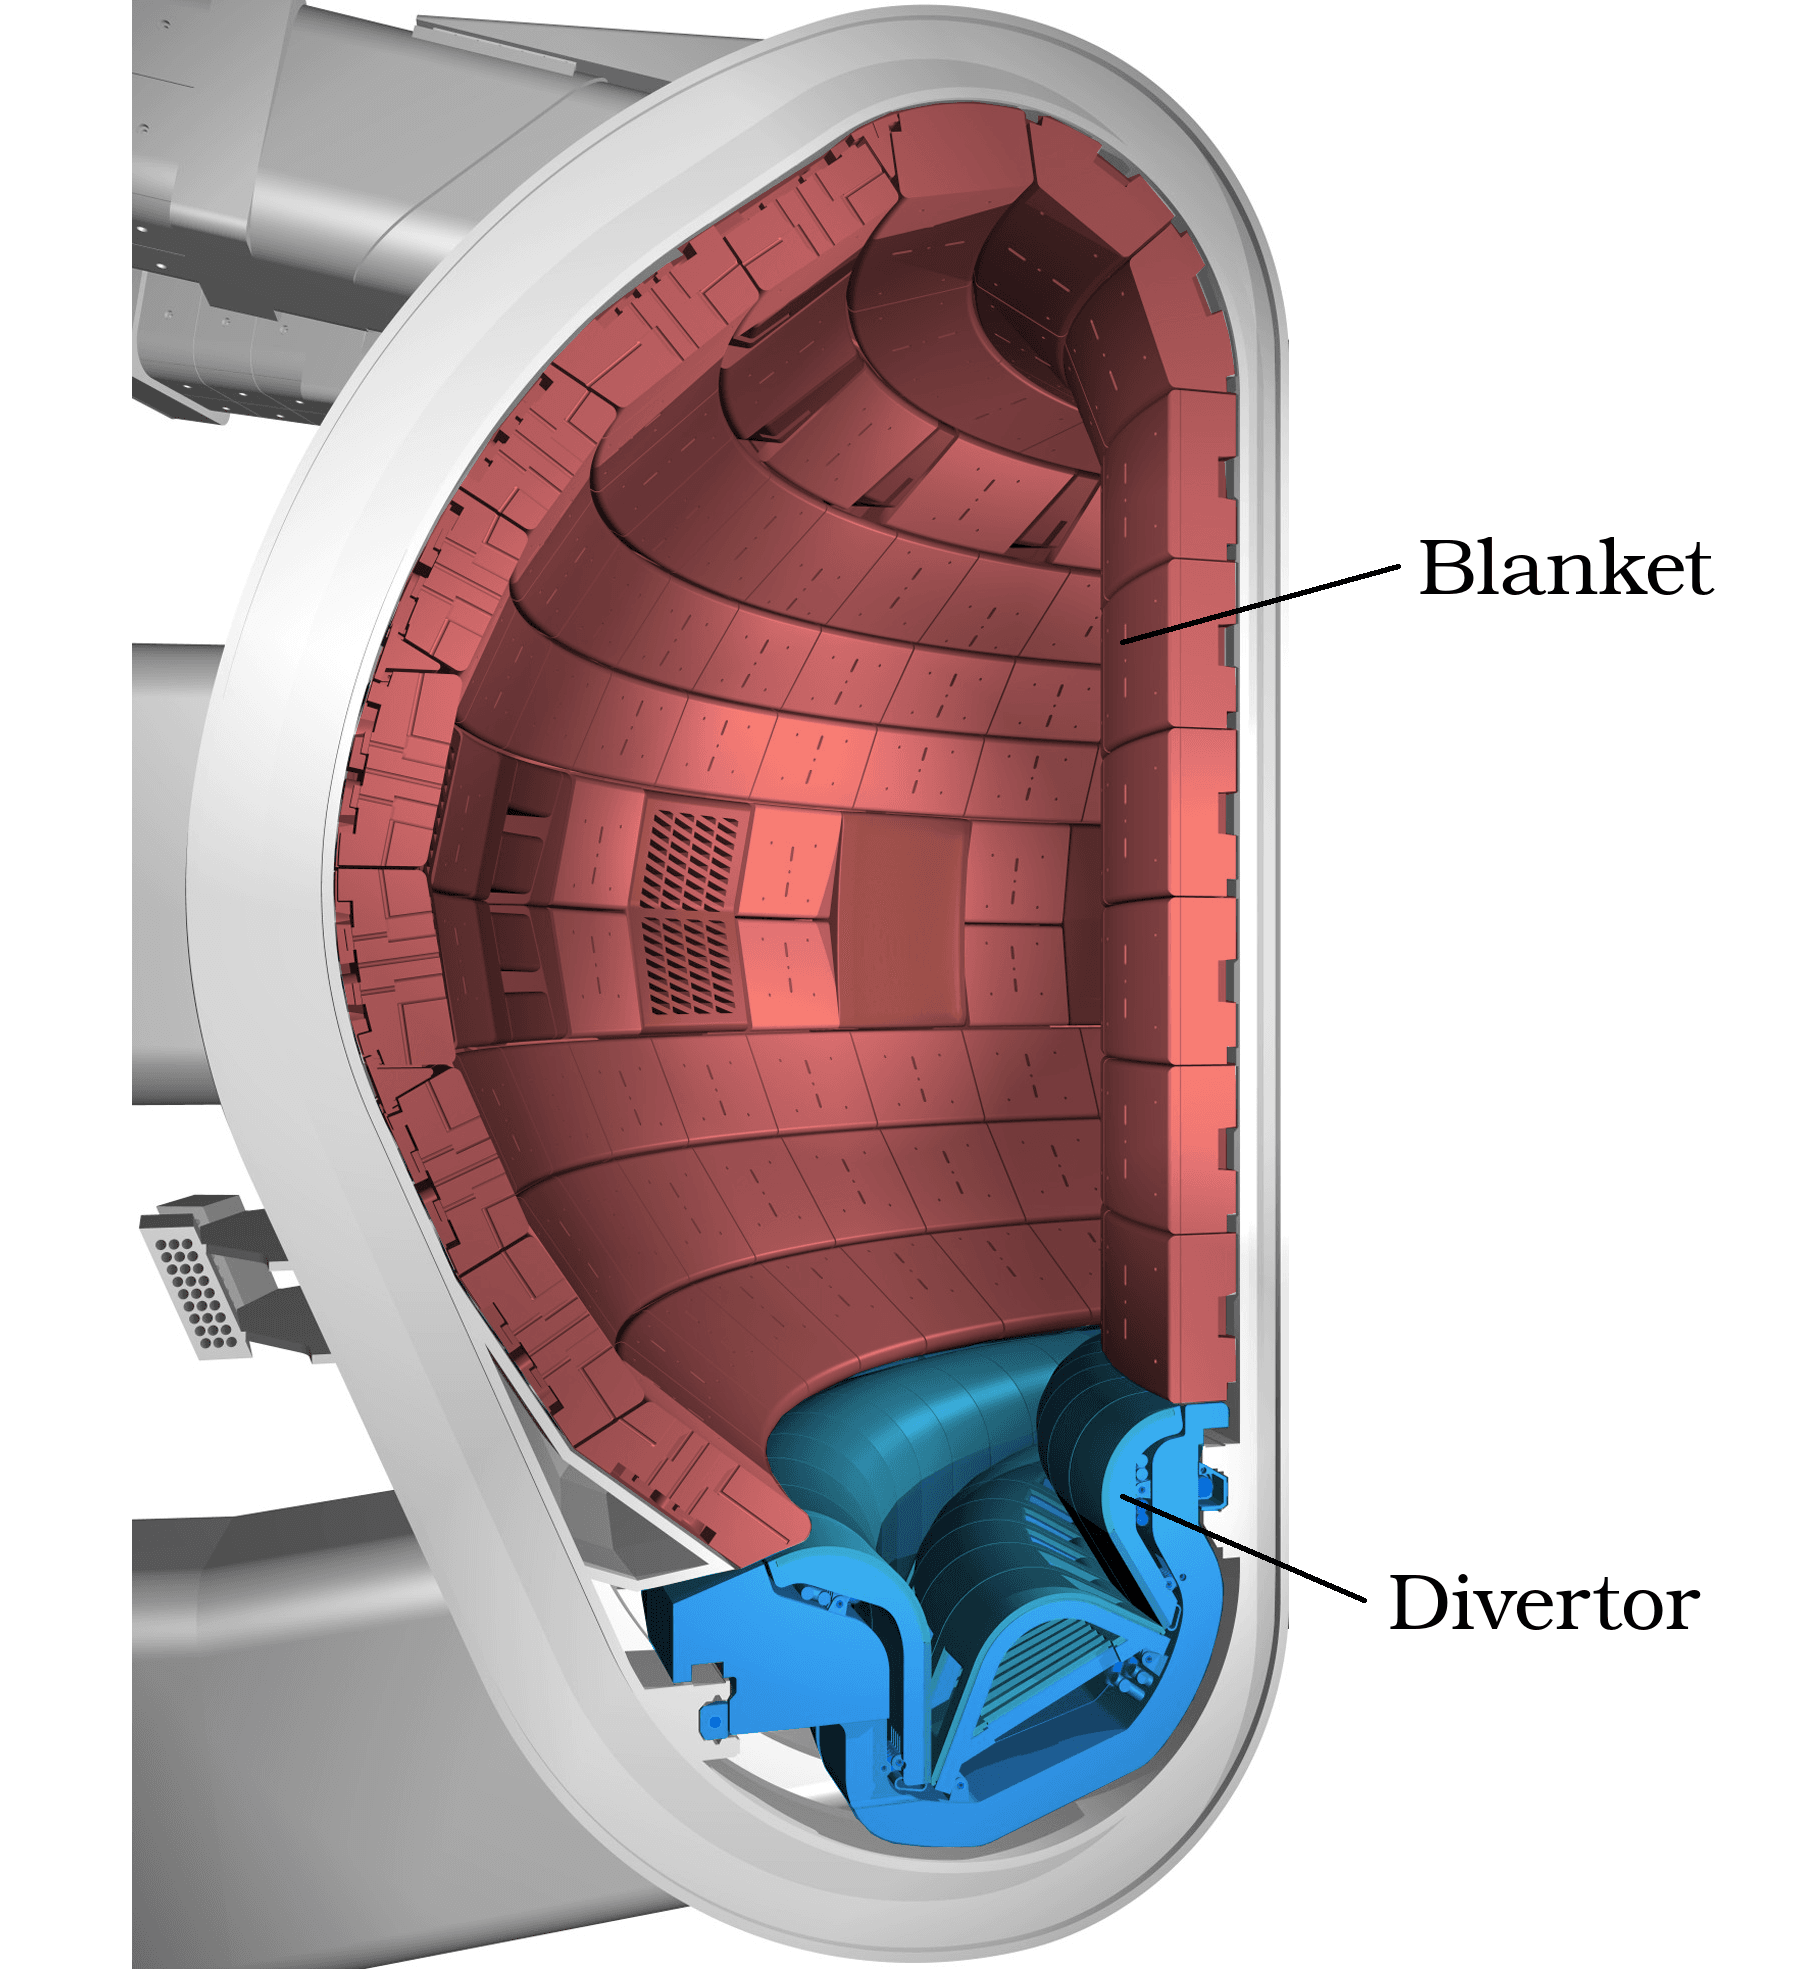
\includegraphics[scale=0.1]{vacuumvessel_edited.png}
\caption{A section of the ITER tokamak with the plasma facing components highlighted. Source: Adapted from \cite{ITERCrossSection}}
\label{fig:ITERslice}
\end{figure}

% ---------------------------------------------------------------------------------------------------
\section{Hydrogen Retention in Tungsten}
% ---------------------------------------------------------------------------------------------------
The armour material of choice for the ITER divertor is tungsten (W) \cite{PITTS2013S48}.
The metal, named after the Swedish word for "heavy stone", is recognized for having the highest melting point of all metals (3695 K) and a hardness superior to that of most steels. 
It also has a thermal conductivity of 173 W/(m·K), equaling around twice that of iron and half that of copper. 
In its structurally most stable form, W has a body-centered-cubic (BCC) crystal structure, with a lattice constant of 3.165 \AA.
Due to its small atomic size, hydrogen is soluble to at least some degree in most transition metals, including tungsten \cite{smith1934occlusion, frauenfelder1969solution}.
The equilibrium position for hydrogen in a perfect W lattice is at the tetrahedral interstitial position (TIS), shown as black dots in Fig. \ref{Fig:bcc}. 

At temperatures $T > 0$ K, any real crystalline materials will contain some amount of crystallographic defects, the most common which are visualized in Fig. \ref{Fig:defect_types}. 
The number of these defects increases with the temperature and as the result of irradiation. 
Defects, being disruptions in the periodicity of a lattice, cause an increase in the potential energy of the atomic system. 
\begin{figure}[!ht]
\center
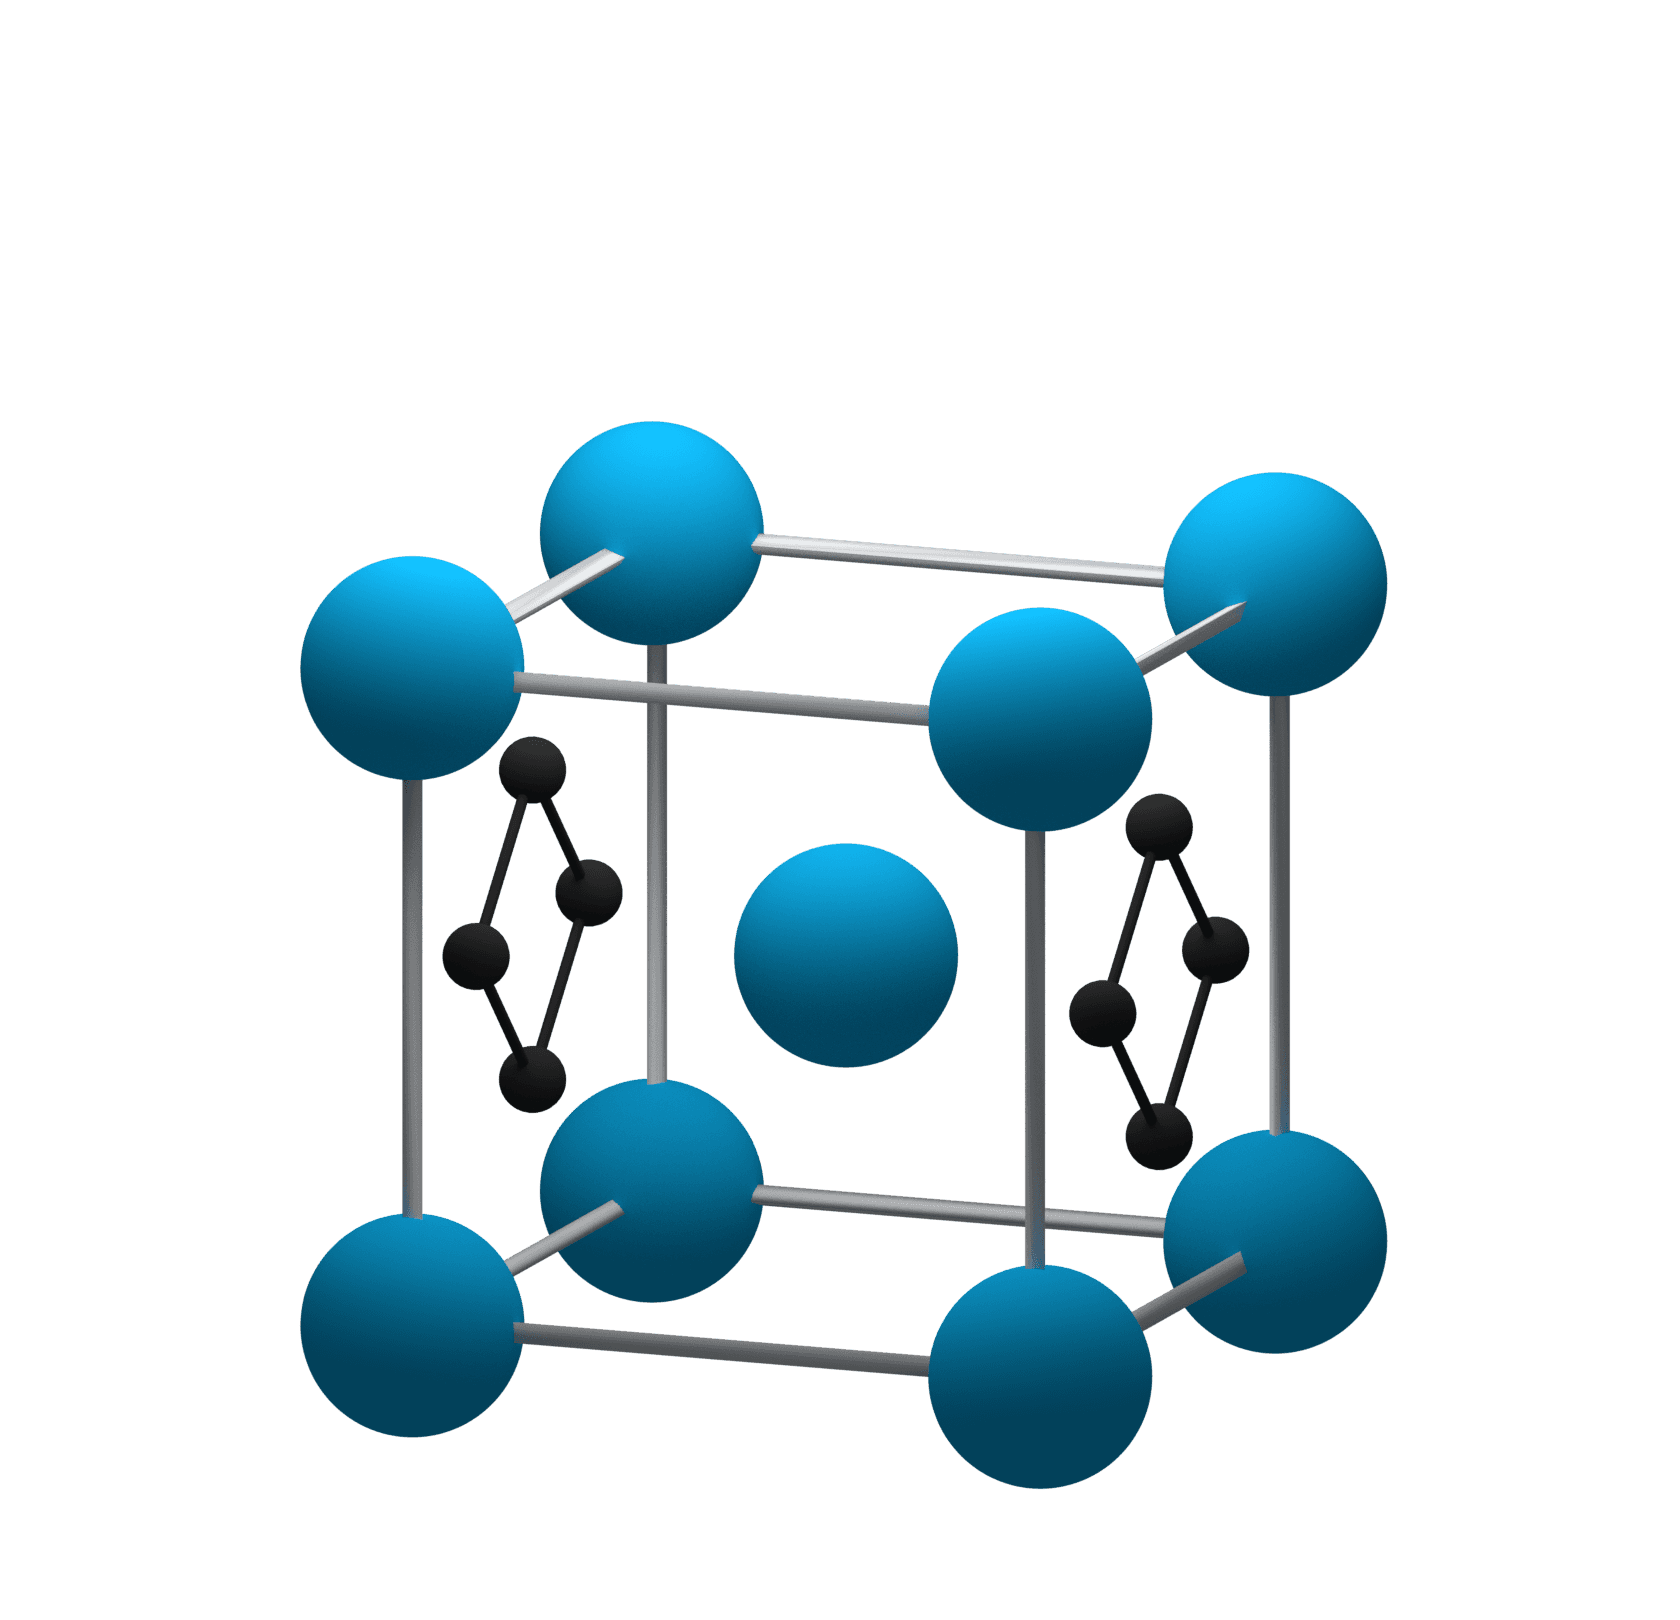
\includegraphics[width=0.3\linewidth]{bcc_render.png}
\caption{The BCC crystalline structure (atoms in blue). Shown in black are 8 out of 24 tetrahedral interstitial positions around the central atom.}
\label{Fig:bcc}
\end{figure}
In a W-H system, formed, e.g. by placing a tungsten object under a hydrogen atmosphere, H atoms tend to lower the system energy by binding to defects. 
E.g. in the case of a vacancy, the empty lattice site leaves neighbouring W atoms with dangling bonds to which hydrogen can bind, leading to a net decrease in energy and six hydrogen atoms being strongly trapped to the defect.

\begin{figure}[!ht]
\center
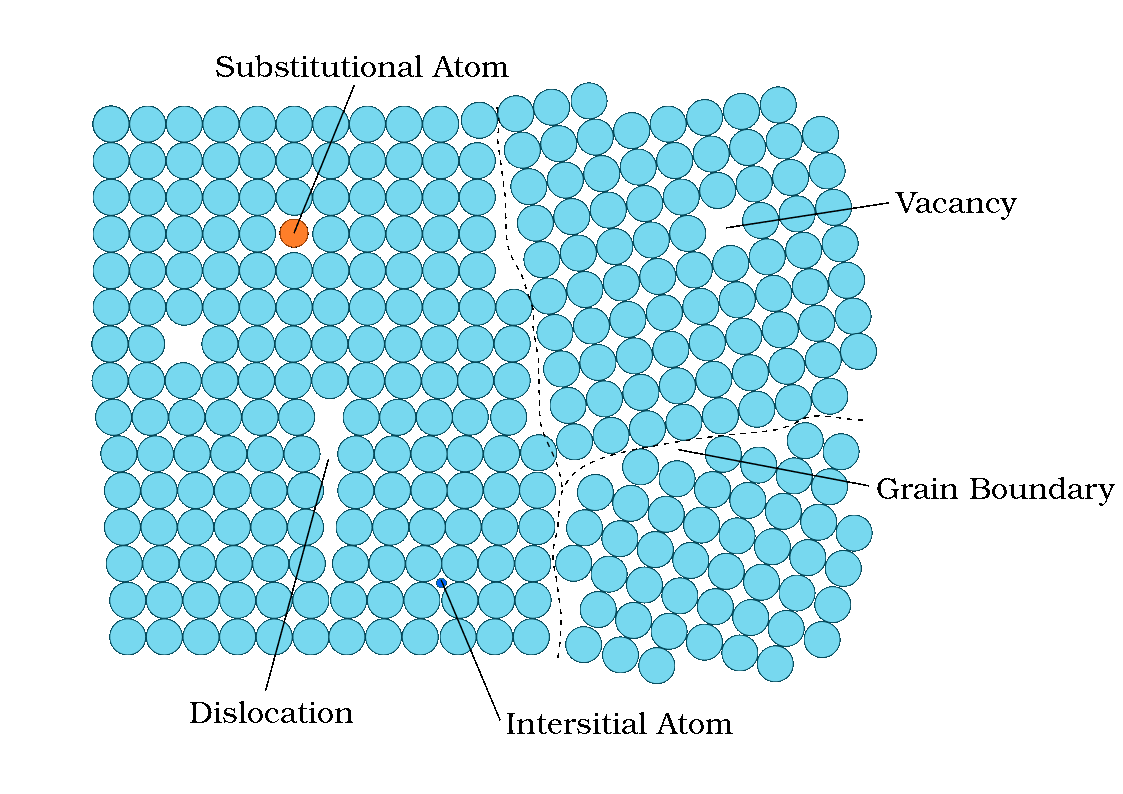
\includegraphics[width=0.76\linewidth]{defect_types.png}
\caption{Various types of crystal defects shown on a 2D lattice}
\label{Fig:defect_types}
\end{figure}


% ---------------------------------------------------------------------------------------------------
\section{Hydrogen Isotope Exchange}
% ---------------------------------------------------------------------------------------------------

The isotopes of a chemical element are essentially variations of the same element, differing in the number of neutrons and thus also atomic mass. 
Since all isotopes of a specific element share the same number of protons and electrons, they can be considered chemically indistinguishable. 
The difference in atomic mass can, nonetheless, present itself as a change in the reaction rates of chemical and thermodynamic processes when an atom is replaced by its isotope. 
Known as the \textit{kinetic isotope effect}, this involves lighter isotopes generally reacting faster than their heavier counterparts \cite{atkins2006atkins}.

In the case of hydrogen, there are three naturally occurring isotopes, protium (H), deuterium (D) and tritium (T). 
In contrast to the vast majority of elements, the relative differences in mass between these three isotopes are notably extreme; D ($m_{\text{D}}=2.014102$ u) and T ($m_{\text{T}}=3.016049$ u) have masses of just over two and three times that of H ($m_{\text{H}}=1.007825$ u). 
These mass differences result in, e.g. the isotopes having noticeably different diffusion rates.

Out of these three isotopes, tritium is the by far scarcest. 
Having a half-life of only 12.3 years, it is formed only in minuscule amounts in the atmosphere through interactions with cosmic rays.
In fusion reactors, where tritium will be present in relative abundance, the trapping of this radioactive substance into wall materials can over time become a safety issue; although tritium is a low-energy beta emitter and thus not externally harmful to humans, it is easily inhaled, ingested or absorbed through the skin, potentially causing radiation damage to internal organs and tissues \cite{tritiumHealth}.
In addition to the safety concern associated with handling and maintaining tritium infused components, there is also an obvious fuel economical incentive of retrieving the embedded tritium.

The proposed methods of detrapping and extracting hydrogen isotopes from materials typically focus on annealing, i.e. heating and slowly cooling a material, to facilitate the detrapping and diffusion of hydrogen atoms. 
Although the rate of diffusion is proportional to temperature as
\begin{align}
D ~\propto~ \exp\left(-\frac{1}{k_{\text{B}}T}\right)
\end{align}
temperatures of above 700 K are still needed to remove the trapped hydrogen within reasonable timescales \cite{heinola2017long}.

This can be partly understood by looking at the binding energy $E_{\text{bind}}$. For the $N$th H atom bound to a defect, this is calculated as
\begin{align}
E_{\text{bind}}(N) ~=~ E(N-1) + E_\text{sol} - [ E(N) + E_\text{bulk} ]
\end{align}
where $E_\text{bulk}$ is the total energy of the perfect crystalline system and $E(N)$ is that of a system with a defect containing $N$ H atoms. 
$E_\text{sol}$, on the other hand, is the energy of a W lattice without the defect, but with a solute H atom at a TIS site.
For most defects, $E_{\text{bind}}$ decreases with $N$, i.e. each added atom is more loosely bound than the previous.
When a hydrogen atom gets detrapped and diffuses far enough from its original position in a defect, it is unlikely to return; either it gets trapped in another nearby defect or eventually exits through an open surface.
As the defect empties this way, it grows increasingly difficult and therefore unlikely for the remaining hydrogen atoms to overcome the $E_{\text{bind}}$ barrier.
In other words, the removal of T from a material slows over time, unless more heat is gradually applied.

Annealing performed under a H$_2$ atmosphere or alternatively under a bombardment of H plasma has, however, been experimentally shown to reduce annealing time or alternatively enable the annealing to be performed at lower temperatures \cite{alimov2011hydrogen, roth2013hydrogen, barton2014deuterium, ahlgren2019hydrogen}.
The mechanism at play here supposedly works by keeping the number of hydrogen atoms bound to a defect constant.  
As a tritium atom now leaves the defect, its place is soon taken by a close-by protium atom, resulting in the low-$E_{\text{bind}}$ states being kept occupied even as the T-removal progresses.
Since hydrogen atoms are assumed to move around somewhat in the defect, the low-$E_{\text{bind}}$ states are shared between the new H atoms and the T atoms remaining in the defect.



%--------------------------------------------------------------------

% ===================================================================================================
\chapter{Molecular Dynamics Simulations}
% ===================================================================================================

% ---------------------------------------------------------------------------------------------------
\section{Molecular Dynamics in General}
% ---------------------------------------------------------------------------------------------------
Molecular dynamics (MD) as a simulation method originates from the 1950s and is, therefore, one of the oldest tools still in use in computational physics and materials research \cite{alder1957phase}.
On a fundamental level, MD consists of solving many-body problems iteratively to determine the forces acting on individual particles. 
These calculations, too complex to have any analytical solutions, are performed using numerical methods and allow us to relatively accurately simulate the dynamic evolution of (semi-)classical systems of particles. 

A typical MD algorithm follows the pattern described in Fig. \ref{MD-schema}. 
The simulation is initiated by giving each atom, $i=1,...,N$, an initial position $\mathbf{r}_i^{(0)}$ and random velocity $\mathbf{v}_i^{(0)}$, consistent with the desired temperature distribution of the system. 
The positions and velocities, $\mathbf{r}_i$ and $\mathbf{v}_i$, are then updated by solving Newton's equations of motion
\begin{align}
\mathbf{F}_i(\mathbf{r}_i,t) = m_i\frac{d^2\mathbf{r}_i}{dt^2} = m_i\mathbf{a}_i(t) = -\nabla_{r_i}V(\mathbf{r}_i)
\end{align}
where $m_i$ is the mass of atom i, positioned at $\mathbf{r}_i$. 
The forces $\mathbf{F}_i$ are determined from the interatomic potential $V(\mathbf{r}_i)$ and can be used to calculate the acceleration of each particle. 
The new positions and velocities are then simply evaluated as functions of the acceleration and the simulation time step $\Delta t$. 
The simulation proceeds through repeated evaluations of the equations of motion, updating the system in increments of $\Delta t$ time units. 
In order to avoid catastrophic errors in the conservation of energy, the time step must be shorter than the inverse vibrational frequency of any process in the system, typically around 1 fs for many materials in equilibrium. \cite{choe2000determination}

% [Neighbour lists & force cutoff]
In its purest form, MD requires us to perform $O(N^2)$ force evaluations, with $N$ being the number simulated of particles. 
In a typical simulation, however, the particles only interact with a limited number of neighbours, and most long-range interactions can be safely disregarded. 
A common way of doing this is by declaring a cutoff radius for the force calculations, with only particles within this radius from particle $i$ taken into account when evaluating $\mathbf{F}_i(\mathbf{r}_i,t)$. 
The use of a force cutoff theoretically reduces the scaling of the algorithm down to $O(N)$. \cite{verlet1967computer}

% [Periodic boundaries] 
Despite the use of a force cutoff, most real-world materials are still far too large to be simulated accurately.
For instance, a typical metal has a number density of around $5\cdot 10^{22}$ atoms/cm$^3$, meaning that simulating even just a $100\times 100 \times 100$ nm$^3$ block of metal, generally considered to be the arbitrary lower limit of bulk materials, would require us to keep track of $5\cdot 10^7$ atoms.
A standard way of cutting corners is through the use of \textit{periodic boundary conditions} (PBCs). 
PBCs imply that particles exiting the region of space confined by the simulation cell borders re-appear on the opposite side, as visualized in Fig. (\ref{Fig:pbcs}). 
Since also interatomic forces are allowed to interact across cell borders, we effectively have a cell surrounded by infinitely many copies of itself.

\begin{figure}[!ht]
\center
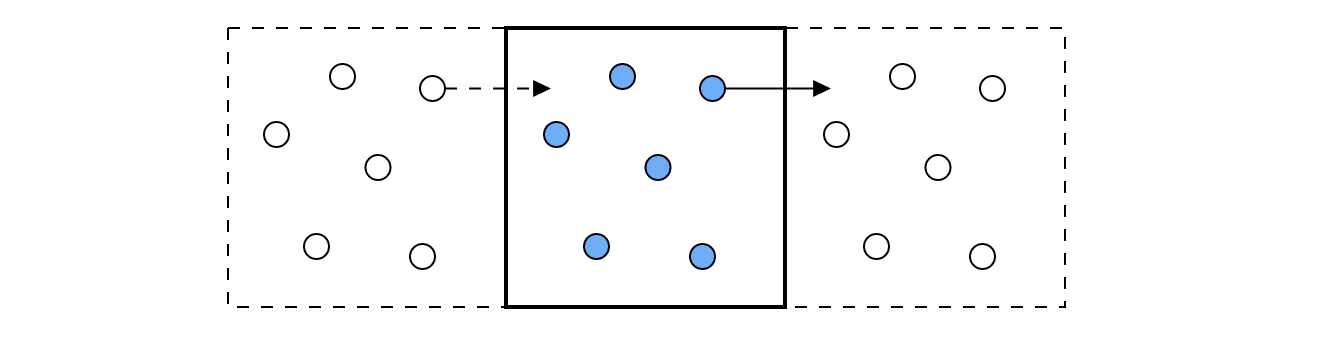
\includegraphics[width=0.75\linewidth]{pbc.png}
\caption{A visualization of periodic boundary conditions in a 2D simulation cell. The cells with dashed lines represent virtual copies}
\label{Fig:pbcs}
\end{figure}

With a perfect lattice, a simulation cell with periodic boundary conditions accurately emulates a bulk material. 
With various defects introduced, we, however, have to make sure that the cell is large enough for the created strain field not to overlap with itself, possibly affecting our results detrimentally.

% [Thermostats, barostats]
Real systems are seldom isolated, but rather exchange at least energy with their surroundings in a number of ways. 
In order to sample a non-isolated thermodynamic ensemble, we need to control the temperature of our simulation manually. 
The temperature of an atomic system is defined as
\begin{align}
T(t) = \frac{1}{k_{\text{B}}N_f}\sum_{i}\left[ m_iv_{i,x}^2(t) + m_iv_{i,y}^2(t) + m_iv_{i,z}^2(t)\right]
\end{align}
where $N_f$ is the number of degrees of freedom and $v_{i}$ is the velocity of atom $i$. 
It is, therefore, straightforward to see why we can control the temperature by scaling atomic velocities.
A common and relatively simple algorithm for this is the so called the \textit{Berendsen thermostat}, defined as
\begin{align}
\frac{dT}{dt} = \frac{T_0-T}{\tau}
\end{align}
where $T_0$ is the target temperature and $\tau$ a time constant. 
Despite its high efficiency, the Berendsen thermostat is not producing a fully correct canonical ensemble and is prone to causing various unphysical artefacts. \cite{berendsen1984molecular}

The \textit{Nos\'{e}-Hoover thermostat}, on the other hand, accurately samples the canonical ensamble. 
Being a so-called \textit{extended system method}, the Nos\'{e}-Hoover thermostat makes use of a virtual particle reservoir, effectively acting as a heat bath. 
Since this requires equations of motions to be evaluated both for the actual particles and the virtual reservoir, the gained physical accuracy comes at a higher computational cost. \cite{nose1984unified}

% --------------- MD schematic ------------------------------------------------------------------------------------
\begin{figure}
\begin{center}
% Define block styles
\tikzset{
decision/.style = {diamond, draw, fill=green!40, 
    text width=4.5em, text badly centered, node distance=3cm, inner sep=0pt},
block/.style = {rectangle, draw, fill=cyan!30, 
    text width=20em, text centered, rounded corners, minimum height=2em},
cloud/.style = {draw, ellipse,fill=red!20, node distance=3cm,
    minimum height=2em}
    }

\begingroup  % compress equations
\medmuskip=2mu
\thinmuskip=1mu
\thickmuskip=2mu
\begin{tikzpicture}
\matrix (m)[matrix of nodes, column  sep=1.5cm,row  sep=5mm, align=center, nodes={rectangle,draw, anchor=center} ]{
    |[block]| {Set initial conditions $\mathbf{r}_i(t_0)$ and $\mathbf{v}_i(t_0)$, set a timestep $dt$ and reset $\mathbf{a}=0$, $_0t=0$}              &  \\
    %|[block]| {\textit{Estimation step:}\\ Estimate new atom positions; \\
    %  Move atoms: $\mathbf{r}_i^{(e)} = \mathbf{r}_i^{(j)} + \mathbf{v}^{(j)}dt + \mathbf{a}\frac{1}{2}dt^2 + ...$\\
    %  Update velocities: $\mathbf{v}^{(e)}=\mathbf{v}^{(f)}+\mathbf{a}dt + ...$}              &  \\
   |[block]| {Calculate $\mathbf{F}_i = -\mathbf{\nabla} V(\mathbf{r}_i)$ and $\mathbf{a}_i=\mathbf{F}_i/m_i$}              &  \\
   |[block]| {Adjust atom positions based on the new $\mathbf{a}_i$;\\
     Move atoms: $\mathbf{r}_i(t_{n+1}) = \mathbf{r}_i(t_n) + f(\mathbf{a}_i,\Delta t)$\\
      Update velocities: $\mathbf{v}(t_{n+1})=\mathbf{v}(t_n)+g(\mathbf{a}_i,\Delta t)$}              &  \\
   |[block]| {Apply boundary conditions, thermostats and barostats as needed}              &  \\
   |[block]| {Calculate and output physical quantities of interest}              &  \\
   |[block]| {$t_{n+1} = t_n+\Delta t$}              &  \\
   |[decision]| {End condition reached?}              &  \\
   |[block]| {Collect data and quit}              &  \\
};
\path [>=latex,->] (m-1-1) edge (m-2-1);
\path [>=latex,->] (m-2-1) edge (m-3-1);
\path [>=latex,->] (m-3-1) edge (m-4-1);
\path [>=latex,->] (m-4-1) edge (m-5-1);
\path [>=latex,->] (m-5-1) edge (m-6-1);
\path [>=latex,->] (m-6-1) edge (m-7-1);
%\path [>=latex,->] (m-7-1) edge (m-8-1);
\draw [>=latex,->] (m-7-1.west) -- node[above] {no} ++(-4,0cm) |- (m-2-1.west);
\draw [>=latex,->] (m-7-1.south) -- node[right] {yes}(m-8-1);
\end{tikzpicture}
\endgroup
\caption{A flowchart representation of a typical Molecular Dynamics simulation. Above, $f$ and $g$ refer to two different functions of the timestep and the acceleration. In the most simple case these would be $f(\mathbf{a}_i,\Delta t) = \mathbf{v}_i\Delta t + \mathbf{a}_i\Delta t^2$ and $g(\mathbf{a}_i,\Delta t) = \mathbf{a}_i\Delta t$, respectively.} 
\label{MD-schema}
\end{center}
\end{figure}
%------------------------------------------------------------------------------------------------------------------


\subsection{Interatomic potentials}

In an MD simulation, potential energies of simulated particles are calculated using so-called \textit{interatomic potentials} -- mathematical functions designed to approximately emulate the interactions between atoms. 
These potentials are usually based upon the Born-Oppenheimer model, i.e. that the electrons of all atoms are permanently in the ground state and that all interactions depend purely on the interatomic distance \cite{born1927quantentheorie}. 
In general terms, the potential energy of an atomistic system can thus be written as
\begin{align}
V_{tot} = \sum_i^N V_1(\mathbf{r}_i) + \sum_{i,j}^N V_2(\mathbf{r}_i, \mathbf{r}_j) +  \sum_{i,j,k}^N V_3(\mathbf{r}_i, \mathbf{r}_j, \mathbf{r}_k) + ...
\label{V_tot-ekv}
\end{align}
where $N$ is the number of atoms in the system and $V_1$, $V_2$ and $V_3$ respectively are one, two and three body terms \cite{potentialsTheory}.

The indices $i$, $j$ and $k$ iterate through the atom positions in three spatial dimensions and can be restricted to $i < j$ and $j < k$ for symmetric interactions such as those encountered in periodic, monoelemental systems. 
The first term of Eq. (\ref{V_tot-ekv}) can be discarded for systems not affected by an external field, and we are hence left with
\begin{align}
V_{tot} = \sum_i \sum_{j>i} V_2(\mathbf{r}_i, \mathbf{r}_j) + \sum_i \sum_{j>i} \sum_{k > j} V_3(\mathbf{r}_i, \mathbf{r}_j, \mathbf{r}_k) + ...
\end{align}
Potentials employing terms of a higher order than two are referred to as \textit{many-body potentials}, while those using only the two first terms are consequently called \textit{pair potentials}.

The atomic structure of metals allows them to be described particularly well using the so-called \textit{Embedded Atom Method} (EAM) formalism, which gives the potential energy in the form
\begin{align}
V_{tot} = \sum_i^N F_i\, \bigg( \sum_j \rho\, (\mathbf{r}_{ij}) \bigg) + \frac{1}{2} \sum^N_{ij} V_2 (\mathbf{r}_{ij})
\end{align}
where  $F_i$ is a function of the summed electron density $\rho (\mathbf{r}_{ij})$ and $\mathbf{r}_{ij}$ denotes the distance $| \mathbf{r}_i - \mathbf{r}_j |$ between the $i$th and $j$th atoms. \cite{EAMmodel,dudarevEAMpotential}. 

For covalently bonded materials, it is often more accurate to use a \textit{Bond Order Potential} (BOP), generally presented as
\begin{align}
V_{ij}(r_{ij}) =bV_{ijk}V_{\rm attractive}(r_{ij}) V_ {\rm repulsive}
\end{align}
Examples of BOPs are potentials of Tersoff, Brenner and Finnis-Sinclair type. \cite{tersoff1988new, brenner1990empirical, finnis1984simple} Both BOP and EAM potentials have the functional shape of a typical pair-potential, but act as many-body potentials due to many-body interactions embedded into their pair-terms.

\section{Parallel Algorithms}
Doubling the side length of a cubical atomic system increases the number of atoms by a factor of eight. 
Correspondingly, the number of necessary force calculations increases by a factor of  8 to 64, depending on the use of neighbour lists.
Since we at any given time only store a minimal amount of vector data per atom, this increase in system size is not a particularily demanding memorywise.
Computationally, however, it is indeed expensive due to the increased number of force evaluations performed every time step.

Interestingly, the nature of MD simulations makes them inherently parallel, allowing the forces for all atoms to be calculated simultaneously. 
This fact can be exploited by dividing the computational load across multiple processing units. 
Parallellisation on $P$ processors can be performed using three principal algorithms; \textit{atom-}, \textit{spatial-} and \textit{force-decompositon}. 
\cite{fincham1987parallel}

The atom-decompositon algorithm includes appointing $N/P$ atoms to each processor and requires \textit{all-to-all} communication of forces between processors and therefore it scales as $O(N)$, independently of $P$. 
The force-decomposition algorithm, on the other hand, divides the cell into three-dimensional boxes, with atoms being re-appointed to the corresponding processor each time they enter a new box. 
This method limits the communication required to only neighbouring processors, giving a theoretical scaling of $O(N/P)$ for largely parallel simulations.
The spatial-decomposition algorithm, finally, involves appointing force calculation loops to separate processors.
This method is fairly non-trivial to grasp and achieves at best a scaling of $O(N/\sqrt{P})$, still lagging behind the spatial-decomposition algorithm in performance. \cite{fincham1987parallel,lammpsMD}

% ---------------------------------------------------------------------------------------------------
% \section{Analysis of the Results}
% --------------------------------------------------------------------------------------------------- 



%--------------------------------------------------------------------

% ===================================================================================================
\chapter{Simulations}
% ===================================================================================================

The molecular dynamics code used in this work was the Large-scale Atomic/Molecular Massively Parallel Simulator (LAMMPS) developed by Sandia National Laboratories \cite{lammpsMD}. 
LAMMPS is a free and open-source code, utilizing the Message Passing Interface (MPI) for running spatially-decomposited parallel MD simulations.
Additionally, LAMMPS also provides a scripting language used to set input parameters and run simulations, but which also contains tools for creating and manipulating simple simulation cells.    

The interatomic potential of choice for our simulations was the W-H-He EAM potential developed by Bonny \textit{et al.} and referred to as 'EAM1' in \cite{bonny2014binding}. 
The W-W interaction part of this potential is the same as 'EAM2' developed by Marinica \textit{et al.} in \cite{marinica2013interatomic}. 
It is well-known for providing elastic constants as well as point defect, dislocation and grain boundary properties in good agreement with Density Functional Theory (DFT) calculations and experiments \cite{bonny2014many}. 
The W-H-He potential referred hereafter to as just 'EAM1', has been shown to relatively accurately recreate the interactions of H with both point defects and dislocations in W \cite{bonny2014binding, grigorev2015interaction}. 

Due to the long in-simulation times, particular attention had to be paid to optimisation of all aspects of the simulations.
The overall computational load could be reduced by scaling down the atomic systems to the bare minima without significantly affecting the accuracy of our results.
For instance, by reducing the side length of a cubic cell of tungsten from 12 unit cells to 10, we have exactly 662 fewer atoms. 
Assuming a linear, $O(N)$, time complexity, this amounts to a 25 \% decrease in wall-time.
On a two-week-long simulation, run in parallel on six CPUs, this small change would mean saving over 500 CPU hours. 

For systems consisting of thousands of atoms, running MD in parallel is imperative, but comes with additional considerations.  
Utilising too few CPUs results in obvious performance issues, while using too many is wasteful and can cause slow-downs due to increased inter-processor communication.
A poorly chosen number of CPUs can additionally result in a suboptimal division of the simulation cell among the processors. 
By using short test runs, we could determine the optimal number of CPUs for each configuration.

% ---------------------------------------------------------------------------------------------------
\section{Simulation Setups}
% ---------------------------------------------------------------------------------------------------
Although the simulations differ largely from defect to defect, a general pattern can be extracted for all of our isotope exchange simulations. 
First, a simulation cell of bulk W containing the defect was created and allowed to reach a minimum energy configuration by first employing numerical minimization and then relaxation through repeatedly heating and cooling the system during short MD cycles. 
The energy minimization method of choice was a Polak-Ribi\`{e}re conjugate gradient algorithm \cite{polak1969note}, which iteratively shifts atom coordinates until a local energy minimum is reached. 

Following the initial relaxation, a large amount of T atoms were deposited at random positions around the cell and allowed to diffuse around during successive MD runs, until the defect had been fully saturated with hydrogen.
After this, the excess T was removed before adding H to random interstitial sites around the cell. 
Isotope exchange was then simulated by running MD for a total simulation time of 100...1450 ns. 

Periodic boundaries were applied in all directions, and the pressure and temperature were controlled using a Nos\'{e}-Hoover thermostat and barostat, emulating an isothermal-isobaric ensemble. 
In a real-world situation, a T atom leaving a defect and diffusing far away would very unlikely return to its starting point, as opposed to getting caught in another defect or leaving the material through a surface. 
Due to the periodic boundaries, however, the T atoms cannot leave the space defined by the cell, as a border-crossing atom merely returns from the opposite side. 
The simulations were therefore performed in intervals of 5 ps (5000 time steps), and after each interval, any T atoms having moved sufficiently far away were automatically removed from the simulation. 
In this scope, 'far away' was defined as a distance $d_{\rm{rmv}} $ from the initial position of the T atom. 
Depending on the geometry of the defect, this parameter had a value of 14...40 \AA, i.e. ca 4...13 unit cells.

As we intend to verify that isotope exchange indeed results in more effective tritium removal than conventional methods, setups for comparison simulations were constructed by omitting the added H and only simulating the spontaneous diffusion of T away from the defect. 
These monoisotopic systems should approximately emulate vacuum annealing conditions.  


% --------------- IsoEx MD ------------------------------------------------------------------------------------
\begin{figure}[!ht]
\begin{center}
% Define block styles
\tikzset{
decision/.style = {diamond, draw, fill=green!40, 
    text width=4.5em, text badly centered, node distance=3cm, inner sep=0pt},
block/.style = {rectangle, draw, fill=cyan!30, 
    text width=12em, text centered, rounded corners, minimum height=2em},
smallblock/.style = {block, text width=7em},
cloud/.style = {draw, ellipse,fill=red!20, node distance=3cm,
    minimum height=2em}
    }
\begingroup  % compress equations
\medmuskip=2mu
\thinmuskip=1mu
\thickmuskip=2mu
\begin{tikzpicture}
\matrix (m)[matrix of nodes, column  sep=0.0cm,row  sep=5mm, align=center, nodes={rectangle,draw, anchor=south} ]{
   |[block] (initI)| {Create simulation cell containing defect} & \\
   |[block] (initII)| {Relax \& Deposit H} & \\
    |[block] (MD)| {Run MD for 5000 steps}          &  \\
    |[block] (DelT)| {Delete T atoms for which $d_i > d_{\text{rmv}}$}          &  \\
%    |[block] (Calcd)| {Calculate $d_i$}          &  \\
%    |[decision] (IsOut)| {$d_i > d_{\rm{rmv}}$?}              &  \\
%       & |[smallblock] (Rmv)| {Remove $i$th T}         &  \\
   |[decision] (IsEnd)| {End condition reached?}              &  \\
   |[block] (End)| {Save results \& quit}   & \\
};
\path [>=latex,->] (initI) edge (initII);
\path [>=latex,->] (initII) edge (MD);
\path [>=latex,->] (MD) edge (DelT);
\path [>=latex,->] (DelT) edge (IsEnd);
%\path [>=latex,->] (MD) edge (Calcd);
%\path [>=latex,->] (Calcd) edge (IsOut);
%\draw [>=latex,->] (IsOut.east) -| node[above, near start] {yes} (Rmv.north);
%\draw [>=latex,->] (IsOut.south) -- node[right] {no}(IsEnd);
%\draw [>=latex,->] (Rmv.south) |- (IsEnd.north);
\draw [>=latex,->] (IsEnd.west) -- node[above] {no} ++(-2,0cm) |- (MD.west);
\draw [>=latex,->] (IsEnd.south) -- node[right] {yes}(End);
\end{tikzpicture}
\endgroup
\caption{A flowchart representation of the isotope exchange simulations. Variable $d_i$ refers to the distance between current and initial point of T atom $i$.} 
\label{Fig:isoExSimus}
\end{center}
\end{figure}


% ---------------------------------------------------------------------------------------------------
\subsection{Vacancies}
% ---------------------------------------------------------------------------------------------------
For the vacancy simulations, a monovacancy was created by removing the middlemost atom of a $10\times 10 \times 10$ unit cell (2000 atom) W lattice.  
In contrast to the larger defects, where the defect was saturated using random diffusion, the small size of the point defect enabled us to manually place T at their natural lowest energy positions.
These positions coincide with the octahedral interstitial sites, forming a square bipyramid around the vacancy \cite{heinolaTungstenDFT}.
A total of 19 H atoms were then deposited to randomly chosen tetragonal interstitial sites around the simulation W lattice, as seen in fig. \ref{Fig:monovac_system}, bringing the (H+T)/W ratio to 0.0125. 
The T/H ratio, on the other hand, was 0.32.

A divacancy system was constructed in a similar fashion by removing two neighbouring W atoms and adding a total of 10 T atoms to the defect.

\begin{figure}[!ht]
\center
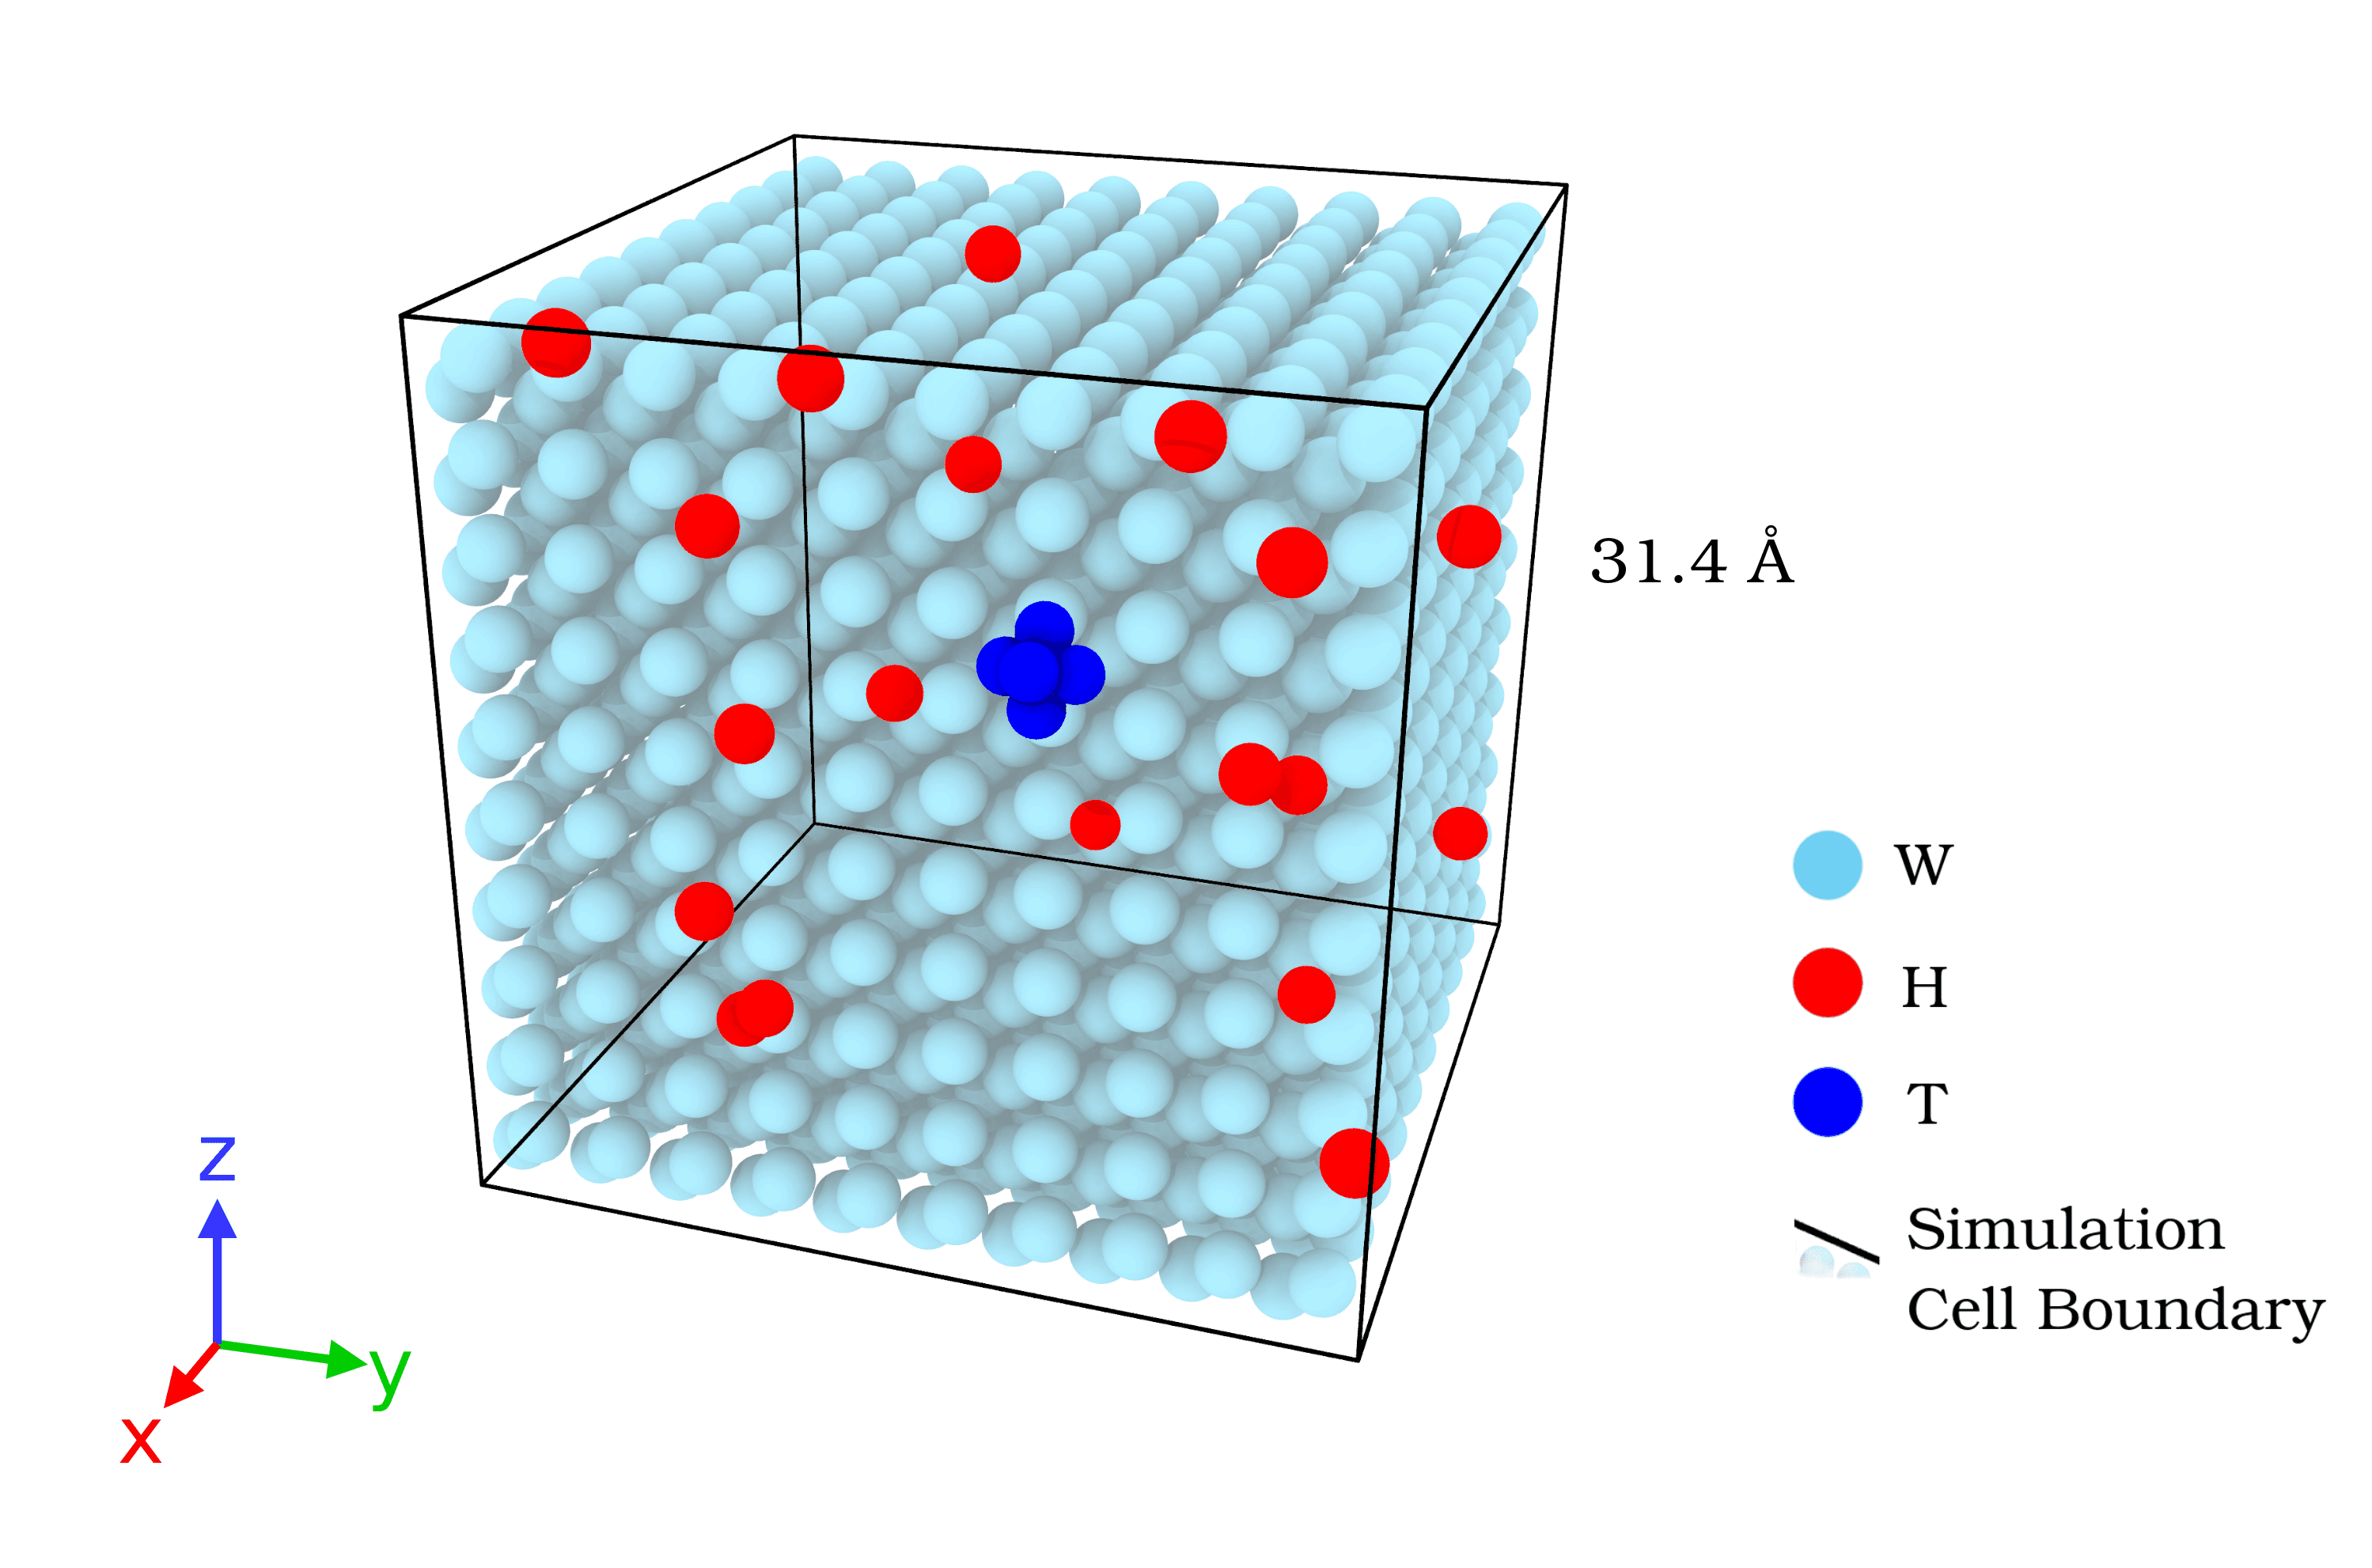
\includegraphics[width=0.7\linewidth]{1Vac_system.png}
\caption{The initial state of the simulation cell used in the monovacancy simulations. 
The W atoms are rendered translucent to display the positions of the hydrogen isotopes.}
\label{Fig:monovac_system}
\end{figure}

% ---------------------------------------------------------------------------------------------------
\subsection{Dislocations}
% ---------------------------------------------------------------------------------------------------
For the dislocation simulations, a  $109.0 \times 136.8 \times 18.4$ $\AA^3$ simulation cell containing a 1/2\hkl[1 1 1]\hkl{1 0 0} edge dislocation was used. 
The defect was generated by first producing a cuboid supercell, with the $x$, $y$ and $z$ axes oriented along the crystal directions \hkl[1 1 1], \hkl[1 1 -2] and \hkl[-1 1 0], respectively, as shown in fig. (\ref{Fig:disloc_system}). 
The cell was then divided into three equally thick slices, parallel to the \hkl{11-2} plane and a dislocation was introduced by inserting a redundant \hkl{1 1 1} atom plane to the middlemost slice, as shown in \ref{ fig:disloc_construction}. 
In order to facilitate the formation of a natural dislocation and to enable the use of periodical boundary conditions, the atom positions in the middle slice were finally compressed slightly.

\begin{figure}[!ht]
\center
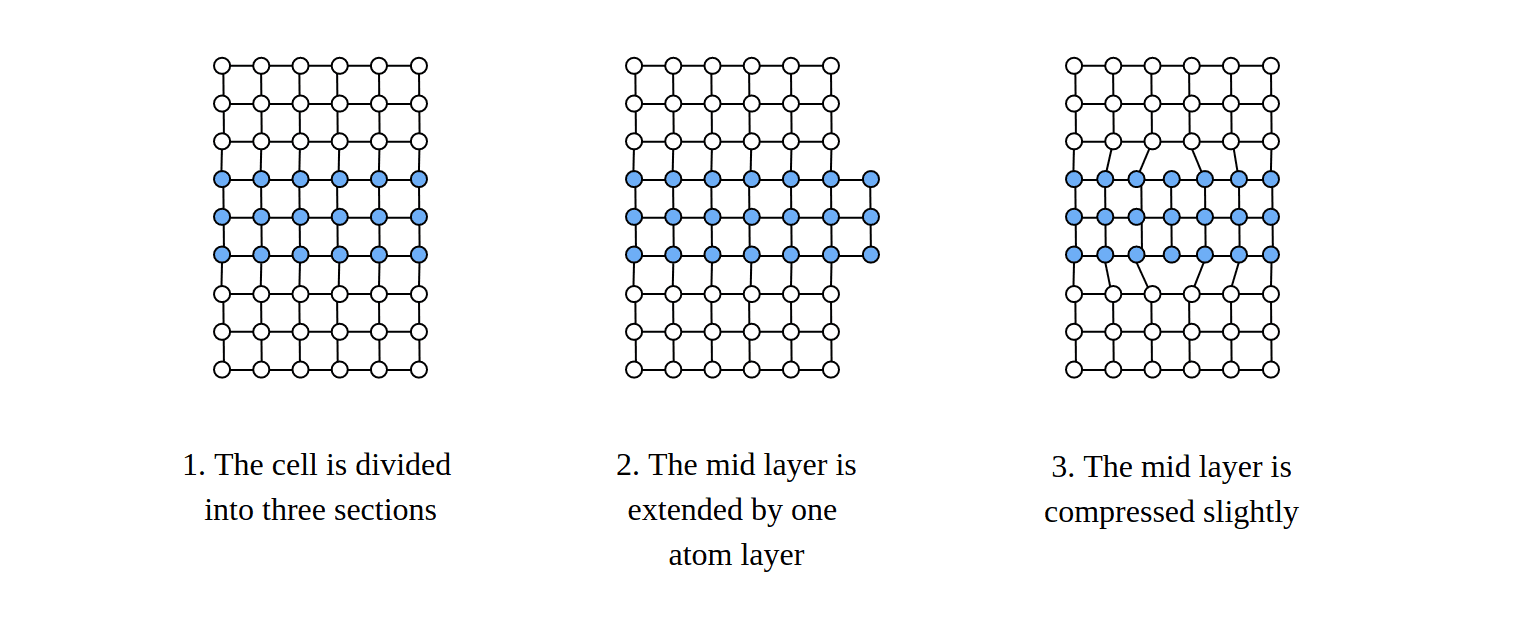
\includegraphics[width=0.85\linewidth]{disloc_construction.png}
\caption{A 2D sketch of the process of constructing the dislocation supercell}
\label{Fig:disloc_construction}
\end{figure}

In practice, the simulation cell was generated using Atomsk \cite{hirel2015atomsk}, an open-source command-line tool for creating and manipulating data files for atomistic simulations. 

\begin{figure}[!ht]
\center
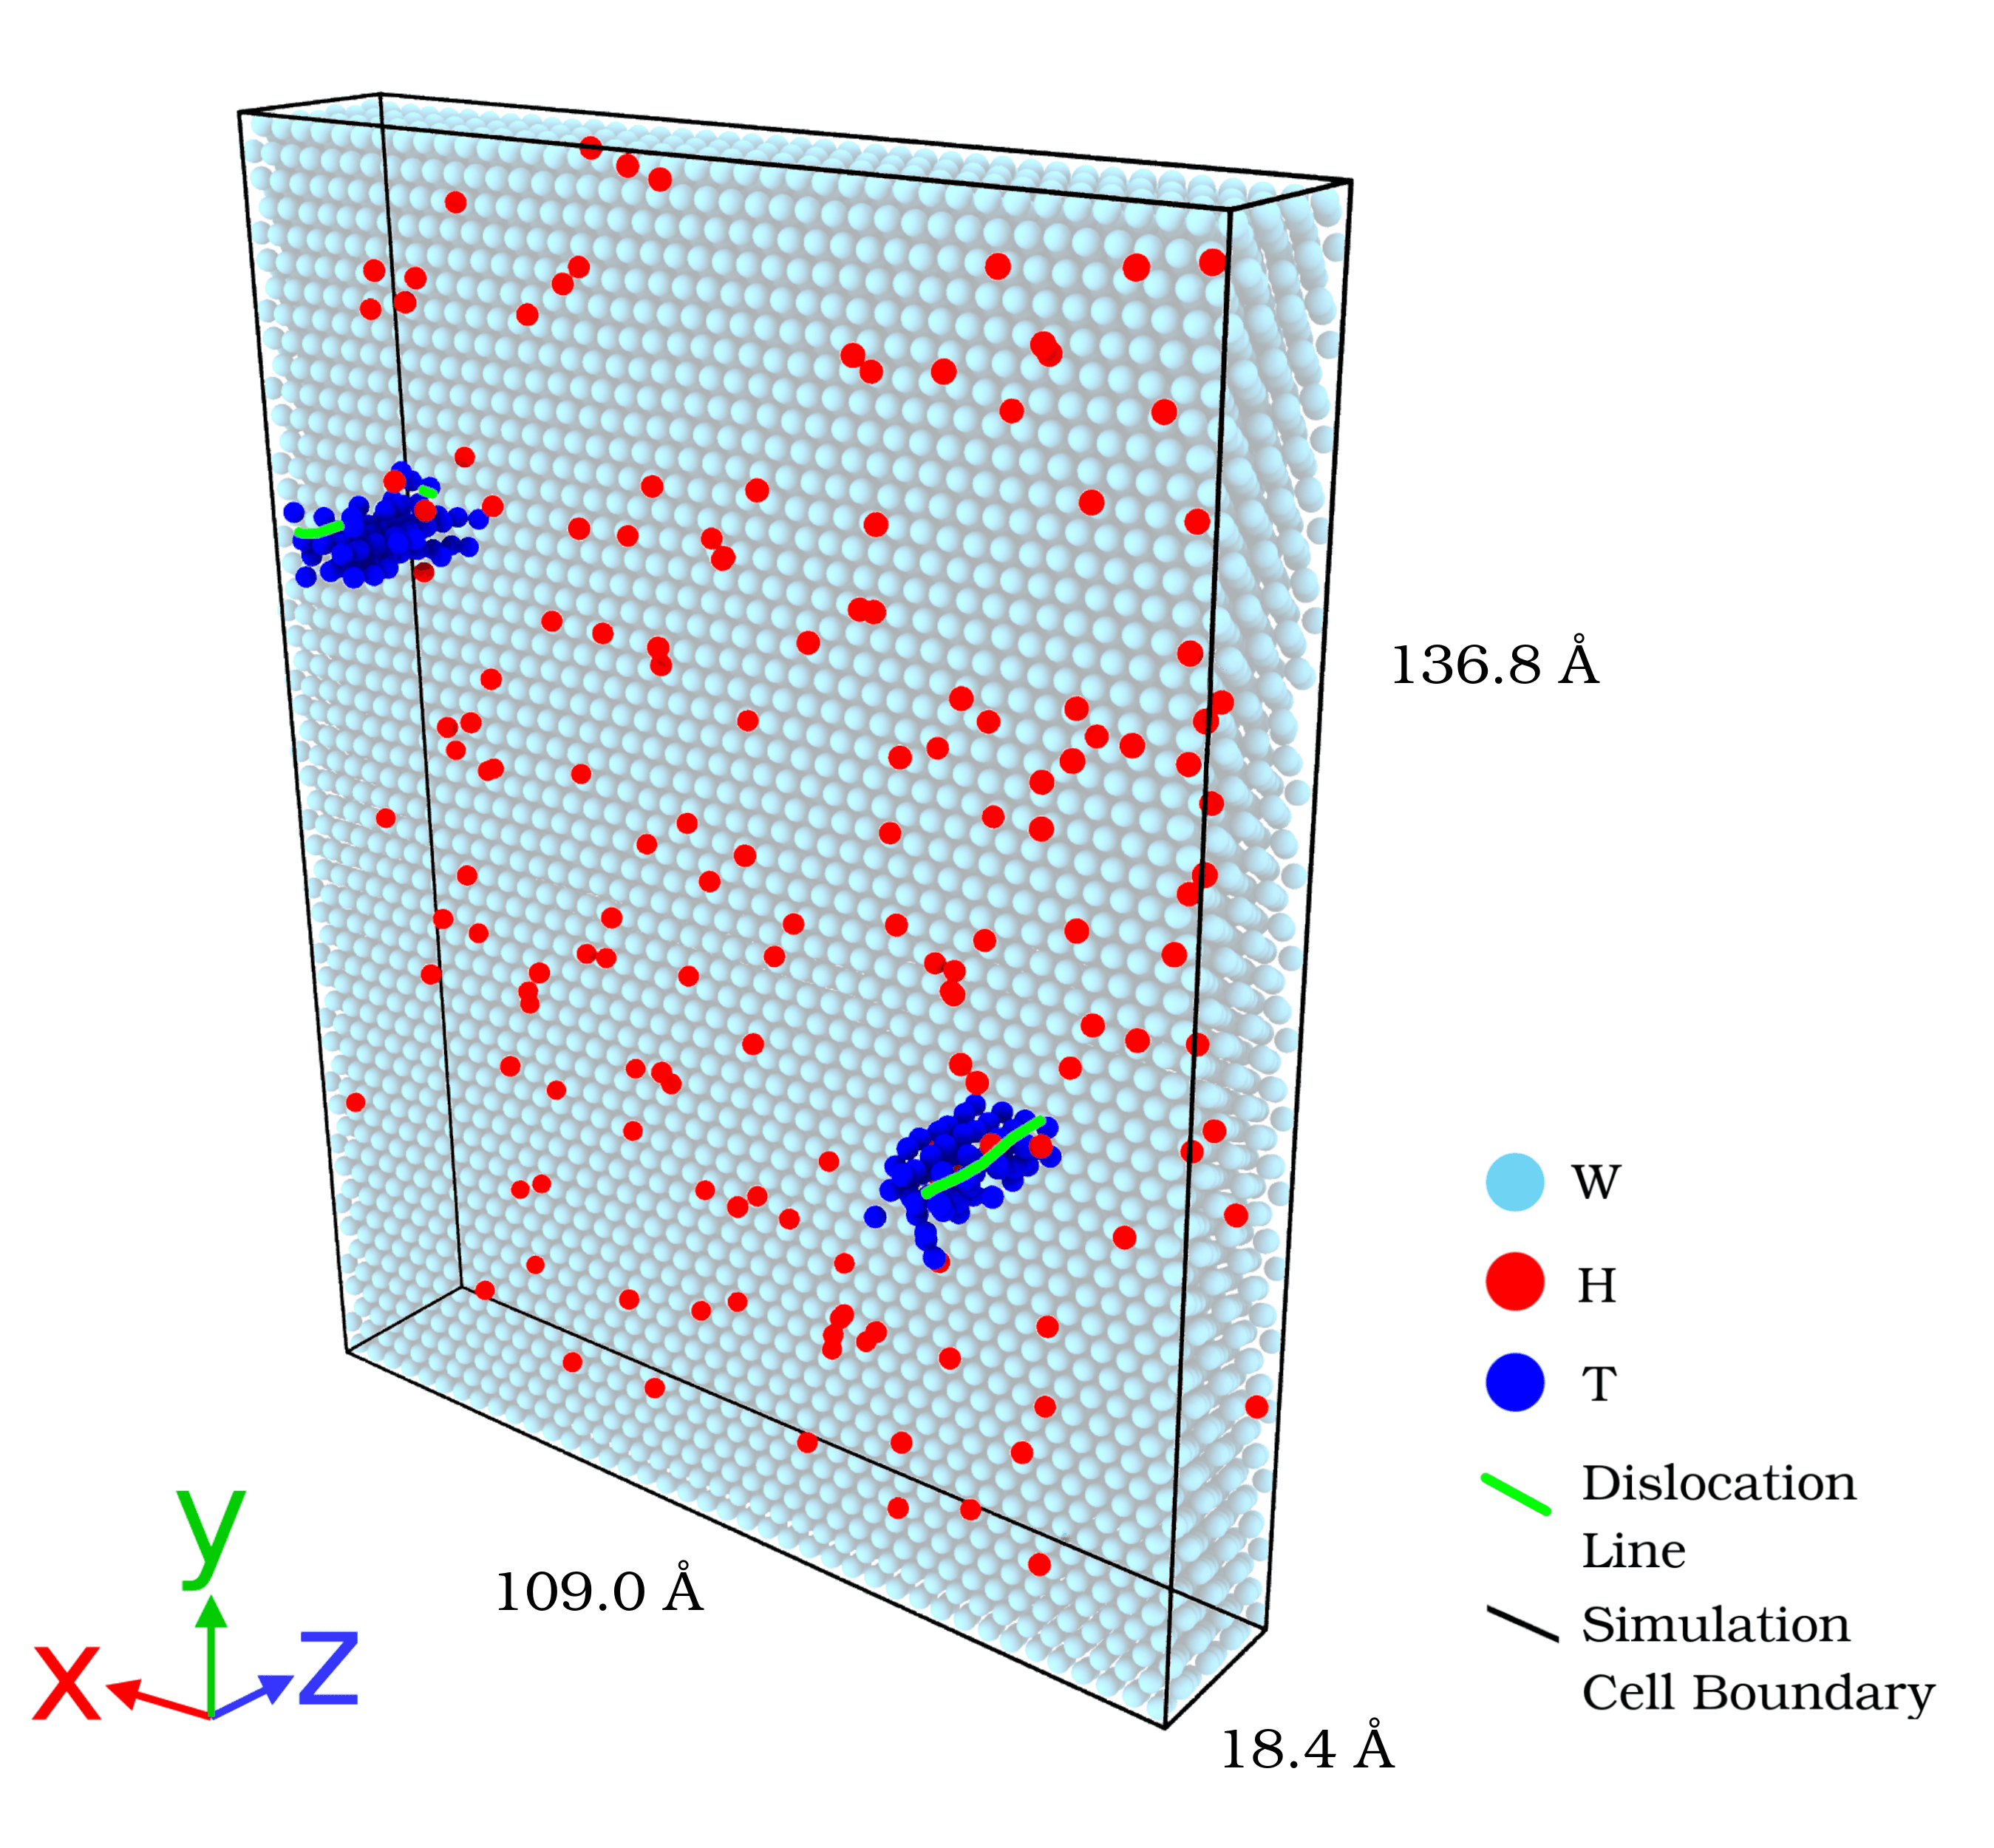
\includegraphics[width=0.7\linewidth]{disloc_system.png}
\caption{The initial state of the simulation cell used in the dislocation simulations. 
The W atoms are rendered translucent to display the positions of the hydrogen isotopes. 
The dislocation, together with its periodic images, is visualized using a defect mesh.}
\label{Fig:disloc_system}
\end{figure}

% ---------------------------------------------------------------------------------------------------
\subsection{Grain Boundaries}
% ---------------------------------------------------------------------------------------------------
% $\Sigma$5\hkl{310}/\hkl[001]
For simulating isotope exchange in W grain boundaries, we used a system containing an arbitrarily chosen \hkl(310)\hkl[001] tilt grain boundary. 
The simulation cell was created by growing together two separate tungsten lattices, each rotated through $\pm18.43^\circ$, respectively, around the $z$-axis. 
As the $x$-axes of the lattices point along \hkl<310> directions, we have a system with a periodicity of $\sqrt{10}~a$ along the $x$- and $y$-axes, and $a$ along the $z$-axis. 
In order to minimize the number of atoms needed to simulate the system we can set $y >> x \approx z$ and again use periodic boundaries.

% Zhou_2009_H_behaviour_in_W_grain_boudnary_FP.pdf

The data file describing the simulation cell was created using Atomsk \cite{hirel2015atomsk} to grow out the intersecting lattices of the two grains from predefined starting points. 
Overlapping W atoms were later manually removed to produce a clean \hkl(310)\hkl[001] grain boundary.

\begin{figure}[!ht]
\center
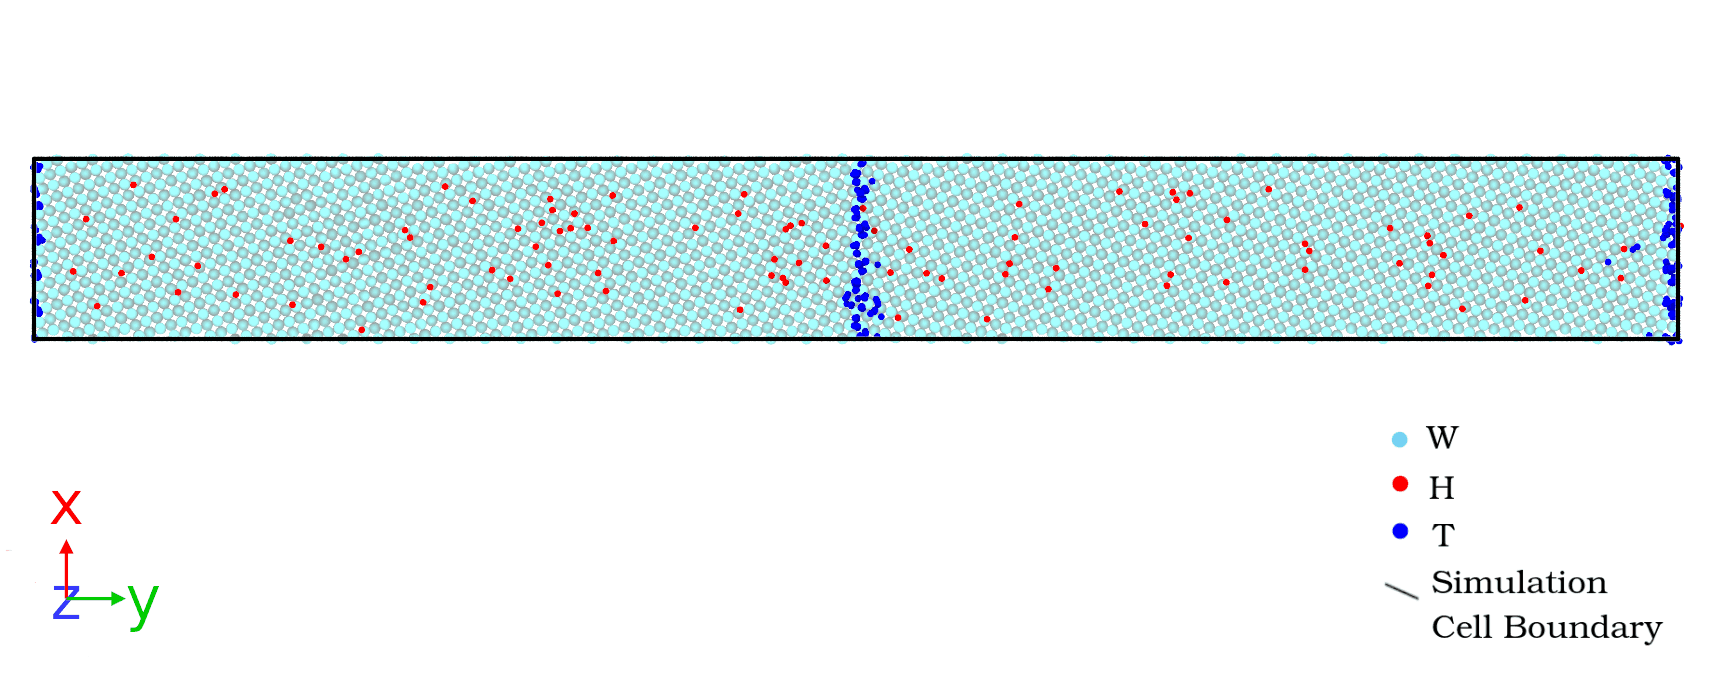
\includegraphics[width=0.94\linewidth]{GB_system.png}
\caption{The initial state of the simulation cell used in the grain boundary simulations. 
The W atoms are rendered translucent to display the positions of the hydrogen isotopes. Break lines are shown to indicate that the cell has been shortened for visual purposes}
\label{Fig:GB_system}
\end{figure}

% ---------------------------------------------------------------------------------------------------
%\section{Impurities}
% ---------------------------------------------------------------------------------------------------



%--------------------------------------------------------------------

% ===================================================================================================
\chapter{Results}
% ===================================================================================================

% ----------------------------------------------------------------------------------
\section{Vacancies}
% ----------------------------------------------------------------------------------
In Fig. \ref{Fig:1Vac_results} and \ref{Fig:2Vac_results} we can see the number of T and H atoms bound to the mono- and divacancies as a function of time, for different temperatures. 
For comparison, the results of the monoisotopic, 'vacuum annealing', simulations are also shown. 
We can see that at all three temperatures, tritium-removal occurs at a higher rate when isotope exchange is involved.
While the difference is more prominent at lower temperatures, it is noticeable also at 500 K, where removal through pure diffusion starts to play a significant role.
Despite us aiming mainly for qualitative results, a semi-quantitative comparison reveals the T-removal rate to be around 50 times higher when employing isotope exchange compared to monoisotopic simulations at 500 K. 

\begin{figure}[!ht]
\begin{subfigure}{.5\textwidth}
  \centering
  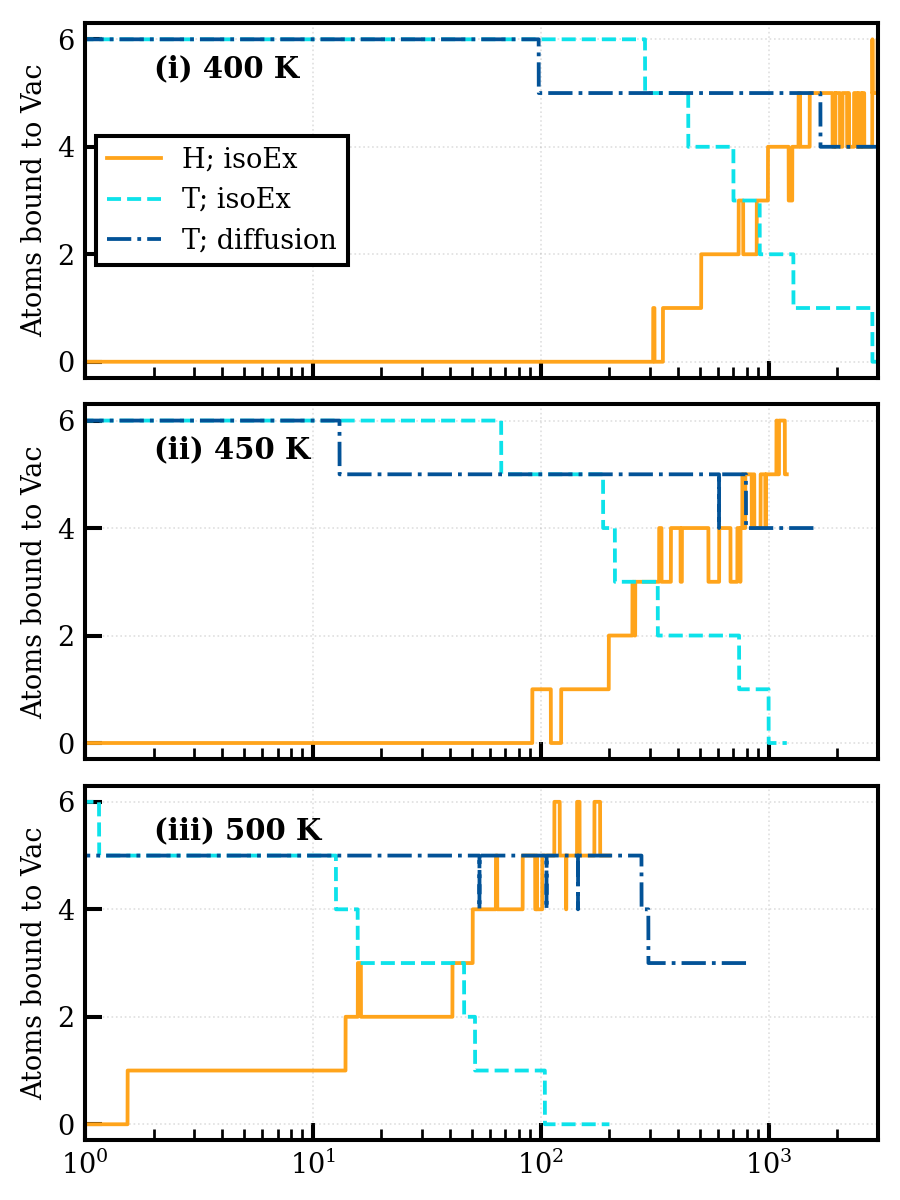
\includegraphics[width=0.99\textwidth]{1Vac_isoEx_HT_log.png}  
  \caption{Logarithmic time scale}
  %\label{fig:sub-first}
\end{subfigure}
\begin{subfigure}{.5\textwidth}
  \centering
  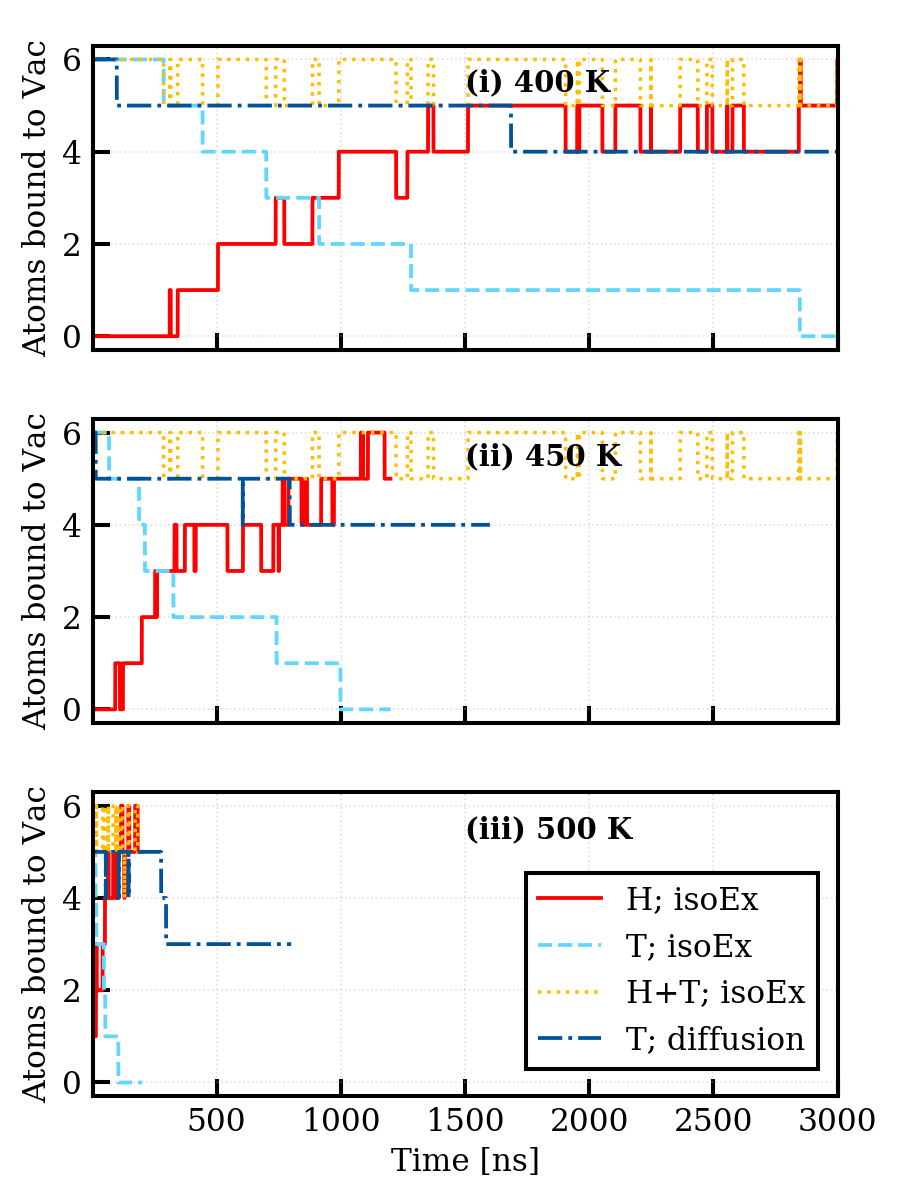
\includegraphics[width=0.99\textwidth]{1Vac_isoEx_HT.png}  
  \caption{Linear time scale}
  %\label{fig:sub-second}
\end{subfigure}
\caption{Number of H and T atoms bound to the monovacancy for isotope exchange and monoisotopic diffusion simulations}
 \label{Fig:1Vac_results} 
\end{figure}


\begin{figure}[!ht]
\begin{subfigure}{.5\textwidth}
  \centering
 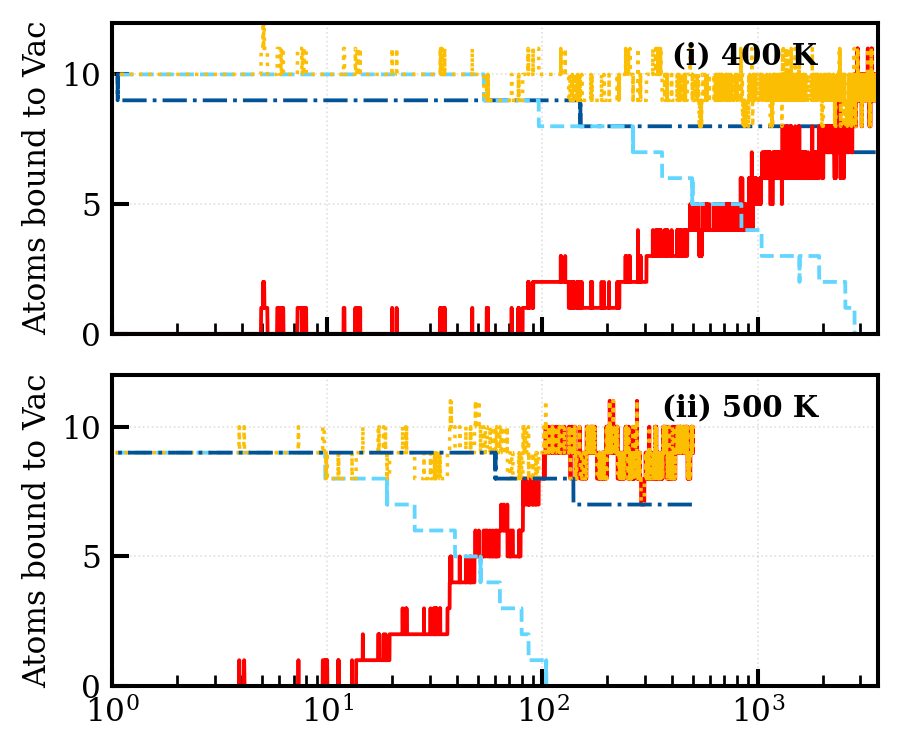
\includegraphics[width=0.99\textwidth]{2Vac_isoEx_HT_log.png}  
  \caption{Logarithmic time scale}
  %\label{fig:sub-first}
\end{subfigure}
\begin{subfigure}{.5\textwidth}
  \centering
  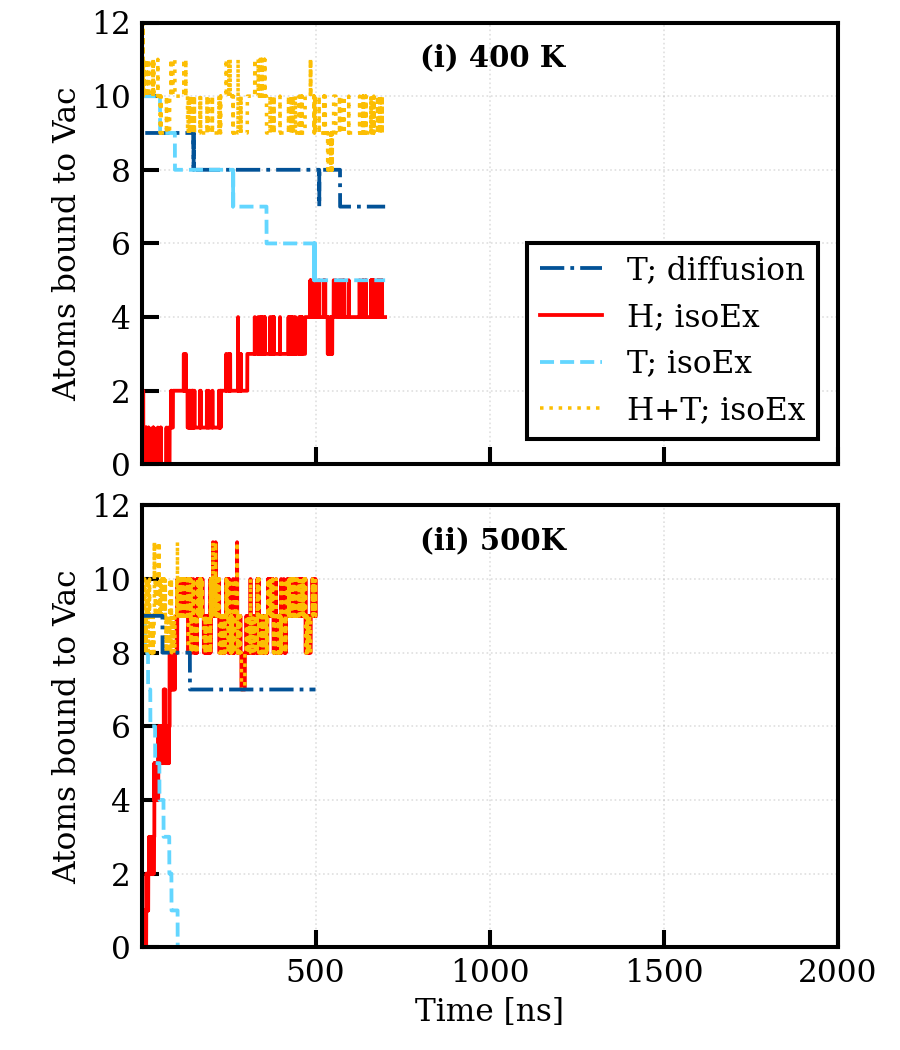
\includegraphics[width=0.99\textwidth]{2Vac_isoEx_HT.png}  
  \caption{Linear time scale}
  %\label{fig:sub-second}
\end{subfigure}
   \caption{Number of H and T atoms bound to the divacancy for isotope exchange and monoisotopic diffusion simulations}
   \label{Fig:2Vac_results} 
\end{figure}

Compared to DFT \cite{heinolaTungstenDFT}, the EAM potential used in this work gives slightly smaller binding energies for the hydrogen-vacancy interaction (Fig. \ref{Fig:Ebind1H_DFT}). 
Absolute tritium removal rates might thus not be directly comparable to experiments, whereas the relative differences between isotope exchange and vacuum annealing simulations are still valid.

Plotting the potential energy of the individual T atoms as a function of time as in Fig. \ref{Fig:Epot}, we can see sharp fluctuations as the atoms move around inside the defect, transitioning in and out of binding energy states.
This seemingly irrelevant fact shows on an atomic level what has been hypothesised based on macroscopic observations to be the basis of the isotope exchange mechanism.
We can also see from both Fig. \ref{Fig:1Vac_results} and \ref{Fig:2Vac_results} that the combined number of T and H in the defects are kept roughly constant during the isotope exchange simulations, with H atoms rapidly taking the place of detrapped T.

\begin{figure}[!ht]
\begin{subfigure}{.48\textwidth}
	\center
	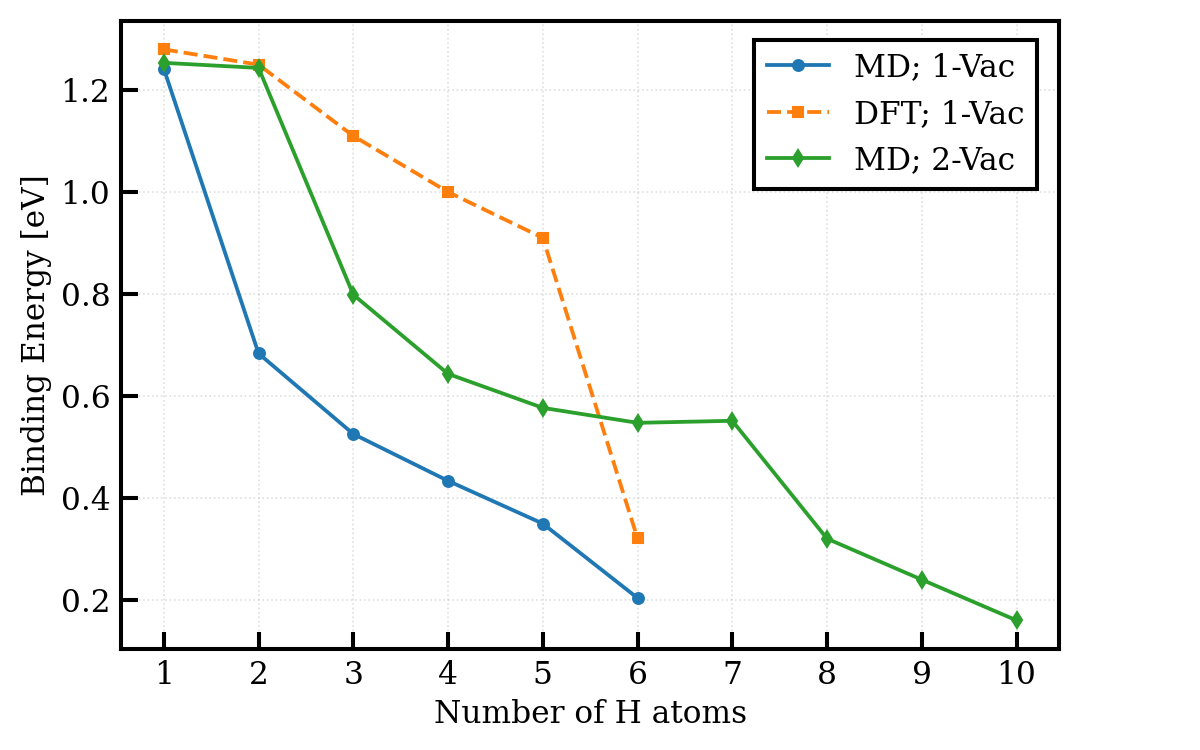
\includegraphics[width=1.1\linewidth]{Ebind.png}
	\caption{Comparision of the H-W binding energy in MD using the EAM1 potential by Bonny \textit{et. al} and DFT results by Heinola \textit{et. al. }\cite{heinolaTungstenDFT}}
	\label{Fig:Ebind1H_DFT}
\end{subfigure}
\hspace{3mm}
\begin{subfigure}{.48\textwidth}
	\center
	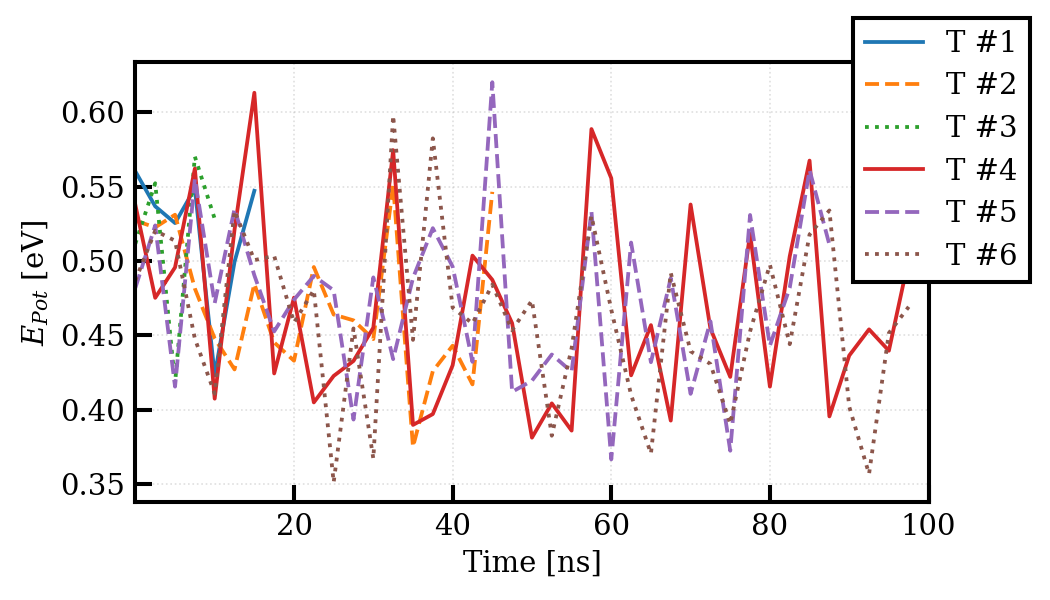
\includegraphics[width=1.1\linewidth]{epot.png}
	\caption{The potential energies of all individual T atoms in a 500 K simulation.\vspace*{6mm}}
	\label{Fig:Epot}
  %\label{fig:sub-second}
\end{subfigure}
\end{figure}


% ----------------------------------------------------------------------------------
\section{Dislocations}
% ----------------------------------------------------------------------------------
The dislocation results are shown in Fig. \ref{Fig:disloc_results} and indicate an enhanced T-removal rate when utilising isotope exchange at 500 K. 
At 400 K, on the other hand, there is no significant difference between the two methods.

Due to the extremely long simulation that would have been required for complete T-removal using the monoisotopic method even at 500 K, we can only state that removal using isotope exchange appears to be several orders of magnitude faster.
 

\begin{figure}[!ht]
\begin{subfigure}{.5\textwidth}
  \centering
 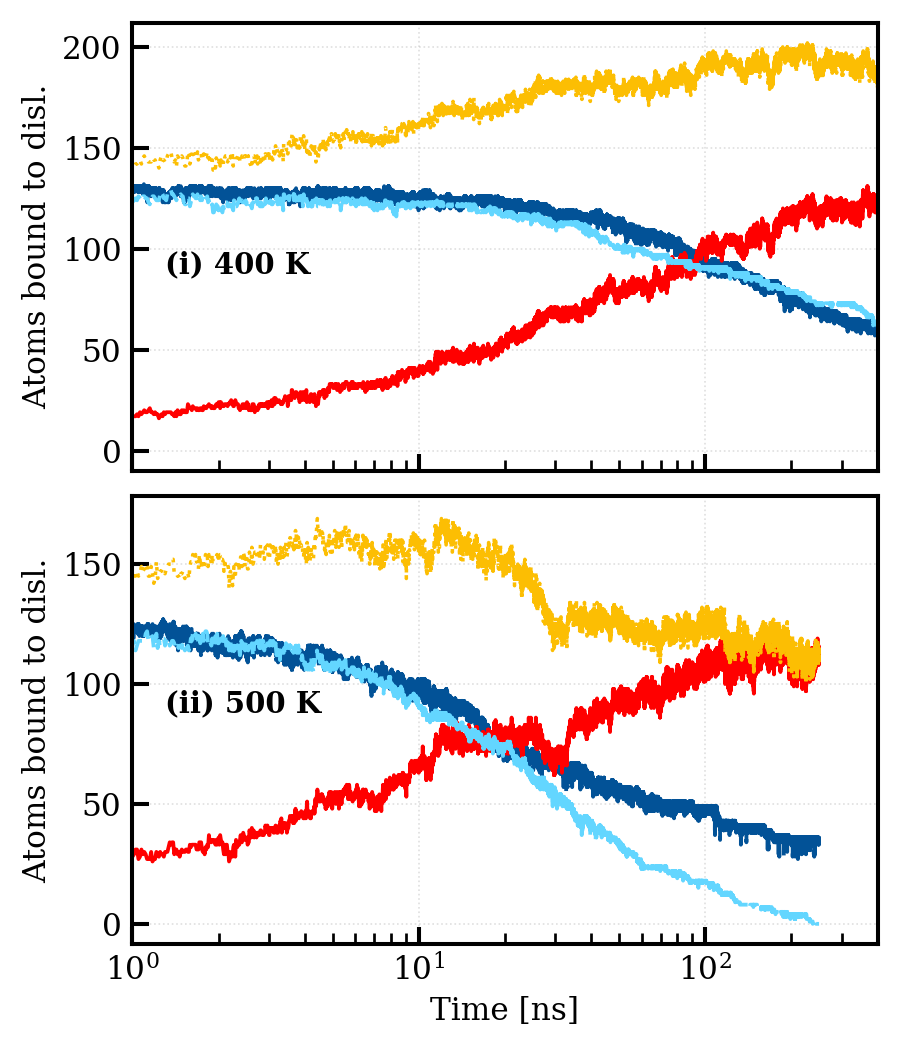
\includegraphics[width=0.99\textwidth]{disloc_isoEx_HT_log.png}  
  \caption{Logarithmic time scale}
  %\label{fig:sub-first}
\end{subfigure}
\begin{subfigure}{.5\textwidth}
  \centering
  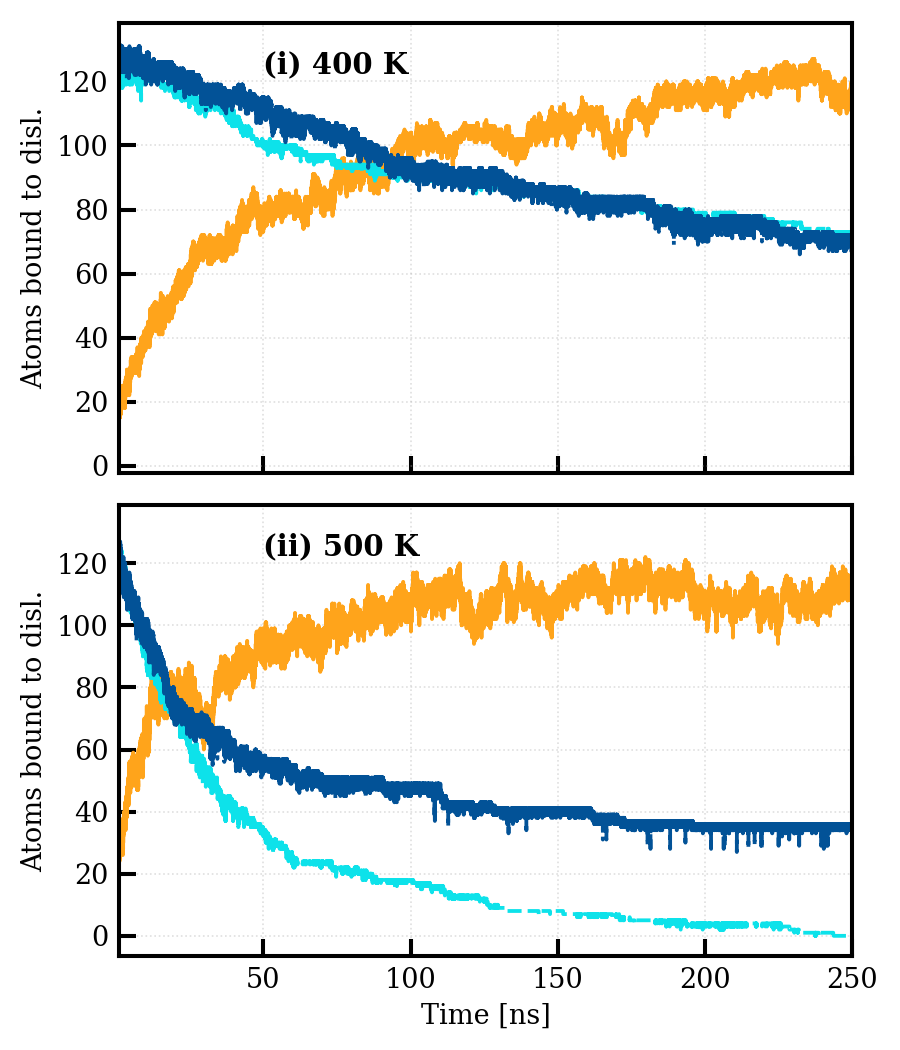
\includegraphics[width=0.99\textwidth]{disloc_isoEx_HT.png}  
  \caption{Linear time scale}
  %\label{fig:sub-second}
\end{subfigure}
   \caption{Number of H and T atoms bound to the dislocation for isotope exchange and monoisotopic diffusion simulations}
   \label{Fig:disloc_results} 
\end{figure}



% ----------------------------------------------------------------------------------
\section{Grain boundaries}
% ----------------------------------------------------------------------------------
The grain boundary results are shown in Fig. \ref{Fig:GB_results}. 
Here, as was the case with the dislocation, an improved T-removal rate can only be observed at 500 K.
Similarly, the exact difference in removal rate was difficult to determine without excessive use of computing resources, but can be clearly seen from Fig. \ref{Fig:GB_results} to be several orders of magnitude higher for the isotope exchange simulations.
The shape of the 


\begin{figure}[!ht]
\begin{subfigure}{.5\textwidth}
  \centering
 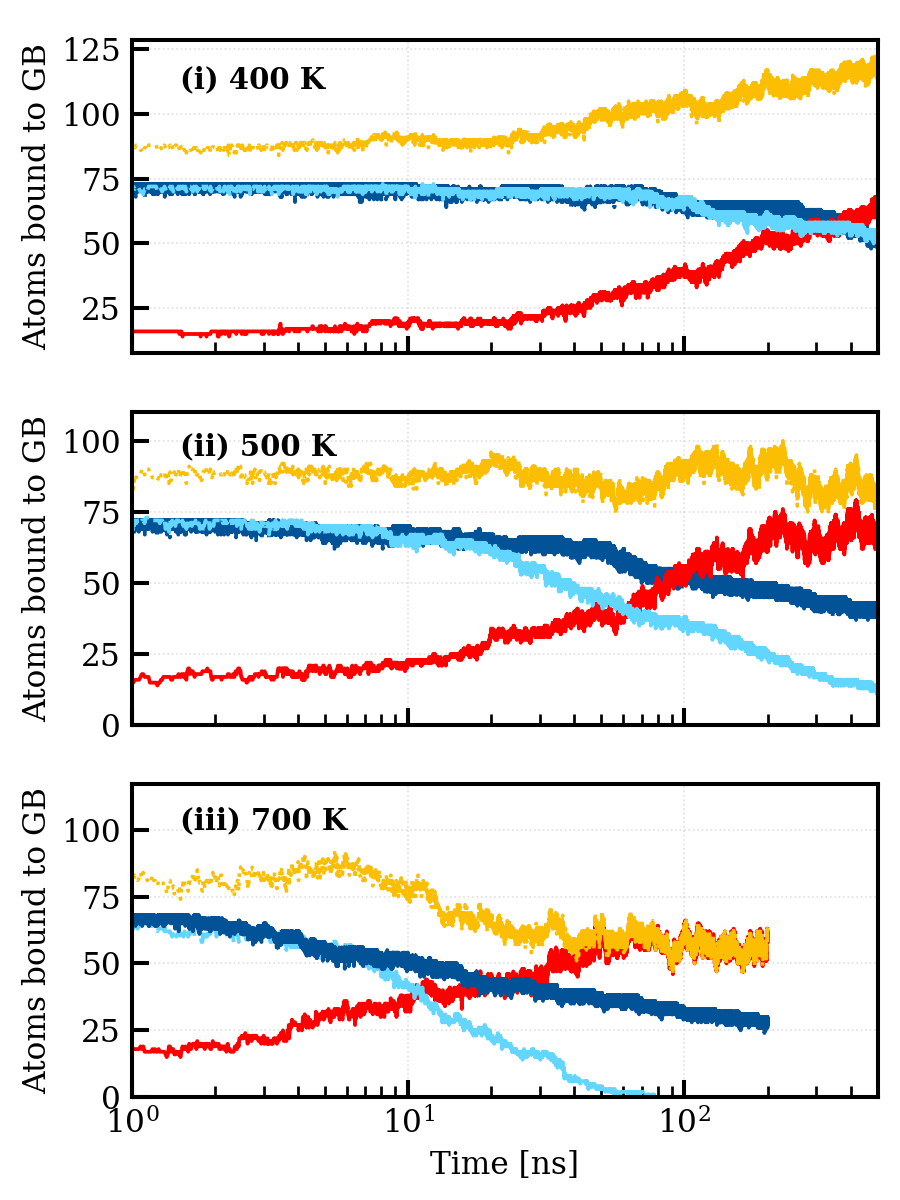
\includegraphics[width=0.99\textwidth]{GB_isoEx_HT_log.png}  
  \caption{Logarithmic time scale}
  %\label{fig:sub-first}
\end{subfigure}
\begin{subfigure}{.5\textwidth}
  \centering
  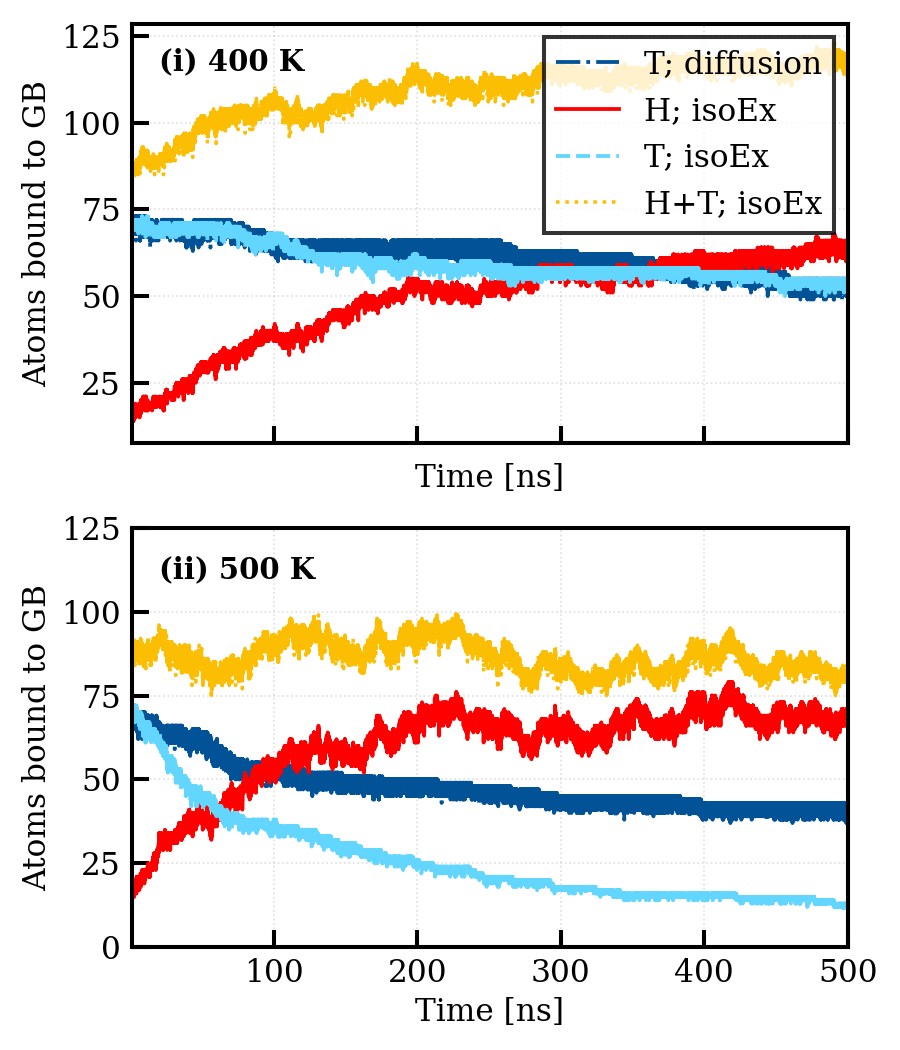
\includegraphics[width=0.99\textwidth]{GB_isoEx_HT.png}  
  \caption{Linear time scale}
  %\label{fig:sub-second}
\end{subfigure}
   \caption{Number of H and T atoms bound to the grain boundary for isotope exchange and monoisotopic diffusion simulations}
   \label{Fig:GB_results} 
\end{figure}



%--------------------------------------------------------------------

% ===================================================================================================
\chapter{Conclusions}
% ===================================================================================================

In this thesis, we have studied hydrogen isotope exchange in crystal defects of bulk tungsten using molecular dynamics. 
Due to their high prevalence in irradiated materials, our simulations targeted hydrogen accumulated into mono- and divacancies, dislocations and grain boundaries.  

Our results indicated significantly improved tritium removal rates for all considered defect types when isotope exchange was employed compared to pure diffusion-based removal methods.
Being well in line with earlier experimental work in the field \cite{ahlgren2019hydrogen}, our results provide an atom-level view into the isotope exchange mechanism, showing that it indeed is based on keeping the defect saturated, with loosely bound hydrogen atoms available through the entire annealing process.

Finally, our results serve to prove that it is possible to study the mechanism of isotope exchange using molecular dynamics methods, despite the limitations it poses on simulation time scales and system sizes.

In the future, the results of this study could be expanded by studying hydrogen isotope exchange around impurity atoms in tungsten.
This would, however, require the existence of a reliable and efficient potential e.g. for a W-H-C system.   


%--------------------------------------------------------------------

% ===================================================================================================
\chapter{Acknowledgements}
% ===================================================================================================



%-------------------------------------------------------------------------------

\cleardoublepage %fixes the position of bibliography in bookmarks
\phantomsection

\addcontentsline{toc}{chapter}{\bibname} % This lines adds the bibliography to the ToC
\bibliographystyle{IEEEtran}
%\bibliographystyle{unsrt} % numbering 
%\bibliographystyle{apalike} % name, year
\renewcommand{\bibname}{References}
\bibliography{bibliography}

%--------------------------------------------------------------------
%\section*{Bilagor}
%\addcontentsline{toc}{subsection}{Bilaga 1}

\end{document}
